\begin{savequote}[9cm]
How do you justify reintegration of Boko haram killers who killed our soldiers and innocent Nigerians back into the society? Are we moving forward or backward?
\qauthor{--- Tweet by \href{https://twitter.com/aelinwa/status/1198636725259644930}{@aelinwa}, 2019}
\end{savequote}


\chapter[How to Forgive Former Fighters?]{How to Forgive Former Fighters?\footnote{This chapter is based on the following article: Godefroidt, A., \& Langer, A. (n.d.). Remorse, Repent and Reconcile: A Conjoint Experiment on Post-conflict Reintegration Attitudes in Nigeria. Revise and Resubmit at \textit{Journal of Peace Research}.}}
\chaptermark{How to Forgive Former Fighters?}
\label{chap:chap3}


\begin{chapabstract}
Which factors foster or impede popular support for the reintegration of particular former members of violent extremist groups? While community acceptance of reintegration is recognized as a \textit{sine qua non} for reintegration to be successful, we still know surprisingly little about the preconditions and circumstances under which community members would be willing to consider reintegrating (particular) former fighters. In order to gain original insights into this important topic, we conducted a conjoint experiment with approximately 2,000 Nigerian young adults. More specifically, we analyzed how reintegration attitudes are shaped by seven features of ex-Boko Haram fighters and tested heterogeneous treatment effects based on three conflict-related characteristics of our Nigerian respondents. Results reveal that, in our study, reintegration attitudes are predominantly driven by signs of remorse, repentance, and reconciliation. These effects seem to operate through respondents’ belief in the success of post-conflict reintegration, and hold for both Christians and Muslims, victims and non-victims, and angry and non-angry respondents. While caution is warranted when generalizing these results, insights gained in this specific geopolitical and historical context may nonetheless be extremely relevant and instructive for other post-conflict reintegration processes.
\end{chapabstract}
\newpage


%----------------------------------------------------------
\section{Introduction}
%----------------------------------------------------------

Reintegrating former fighters, particularly when they have joined so-called terrorist organizations, is a controversial undertaking often causing a public backlash \citep{Schuurman2016, Renard2018}. For example, on 25 July 2020, the Nigerian army announced that about 600 ex-Boko Haram members would be re-integrated back into society \citep{Ogunlade2020}. This decision caused widespread concern across Nigeria, and many Nigerians expressed fierce opposition against it via media messages and protests \citep{Vanguard2020, Vanguard2020a}.\footnote{The Tweet opening this Chapter also illustrated this concern.} Nigeria is not the only country facing this challenge, however. In the last few years, many fighters disengaged from the Islamic State of Iraq and the Levant (ISIL) in the Middle East, the Taliban in Afghanistan and Pakistan, or the Revolutionary Armed Forces of Colombia (FARC). As a result, various governments and communities worldwide are currently struggling with the question what to do about these ex-fighters \citep{Speckhard2020, Steadman2020}. 


Notwithstanding manifold challenges, the conflict resolution and peacebuilding literature has long argued that successfully reintegrating ex-combatants is fundamental to preventing conflict recurrence and building sustainable peace \citep{Knight2004}. As a result, previous work has extensively evaluated the reintegration trajectories of ex-combatants and demonstrated how post-conflict reintegration is extremely complex, multidimensional, and context-dependent (e.g., Gilligan, Mvukiyehe \& Samii, \citeyear{Gilligan2012}; Knight \& \"{O}zerdem, \citeyear{Knight2004}; United Nations, \citeyear{UN2014}; see also Tellez \citeyear{Tellez2019a} for a similar argument). Social reintegration, in particular, poses unique challenges caused by the interactions and relationships between the ex-combatants and community members \citep[][p. 133]{Kaplan2018}. Interestingly, although community acceptance of ex-combatants is often recognized in this respect as a \textit{sine qua non} for social reintegration to be successful, it is rarely addressed in-depth. Moreover, what we know is predominantly based on descriptive accounts or perceptions of acceptance reported by the ex-combatants themselves \citep[e.g.,][]{Humphreys2007, Pugel2007}. Consequently, existing scholarship can tell us little about the conditions and circumstances under which civilians would be more open to allow (certain) former fighters to return to society.


%The Tweet opening of this chapter is part of a growing concern around the world about the reintegration of former members of violent extremist groups.\footnote{To reduce repetition, we use the terms `ex-combatants', `former/ex-fighters', and `former members of violent extremist groups' interchangeably.} As the disarmament, demobilization, and reintegration (DDR) literature has consistently shown, reintegrating ex-combatants back into societies is extremely complex, multidimensional, and context-dependent (e.g., Gilligan, Mvukiyehe \& Samii, \citeyear{Gilligan2012}; Knight \& \"{O}zerdem, \citeyear{Knight2004}; United Nations, \citeyear{UN2014}; see also Tellez \citeyear{Tellez2019a} for a similar argument). While DDR programs seem to be effective to some extent in achieving economic reintegration \citep{Blattman2016}, we know less about the determinants of social reintegration and what we know is predominantly based on descriptive accounts or research with ex-combatants. Yet, whether the public is willing to accept policies allowing former fighters to return home is critical for reintegration to be successful \citep{Kaplan2018}. At the same time, one might expect public resistance against post-conflict reintegration, especially in contexts characterized by extremist and/or terrorist violence. The large-scale campaigns of violence against civilians which such extremist groups often employ, for example, usually feed and strengthen resistance among community members \citep{Abrahms2020}. It is surprising in this respect that, so far, relatively little research has been conducted on the preconditions and circumstances under which community members would be willing to consider reintegrating former fighters. We therefore ask in this chapter: \textit{Which factors foster or impede people's willingness to reintegrate former members of violent extremist groups back into society?}


We study this important issue in a fairly understudied context using a novel methodological approach. More specifically, we conducted a conjoint experiment with about 2,000 Nigerian young adults. The respondents were surveyed by means of a web self-administered questionnaire in-between November and December 2018, and our 2018-survey constitutes one wave within a larger longitudinal study that started in 2015 across Nigerian universities. Although the Nigerian authorities brand their deradicalization and reintegration program as a success, sporadic outbreaks of protest and even violence against ex-Boko Haram members tell a different story. We now build upon these stories by systematically exploring reintegration attitudes from the perspective of the receiving communities. Respondents were presented pairs of hypothetical ex-Boko Haram members and were then asked two questions: (a) which ex-fighter they would prefer to reintegrate back into the Nigerian society and (b) how successful they thought the reintegration process of both ex-fighters would be. Building on peace research and conflict resolution literature, we varied an array of ex-combatant characteristics and, drawing more on political psychology, we also tested heterogeneous treatment effects based on several conflict-related respondent characteristics. By doing so, we integrate several strands of research and propose a more complete typology of post-conflict reintegration attitudes. 


Our analyses yield three main findings. First, we identify key dimensions related to the returning ex-fighter that drive popular support for reintegration. In general, our Nigerian respondents were more willing to reintegrate former Boko Haram fighters who had been forced to join the group, who had fled Boko Haram out of remorse or disappointment with its ideology, and who had undertaken specific reconciliatory acts (especially actively helping the police and military in their fight against Boko Haram). In contrast, they were significantly less willing to reintegrate ex-combatants who had joined the insurgency out of religious beliefs, who had been captured by the military or were forced to leave Boko Haram due to injury or hospitalization, and who did not show any willingness to reconcile. Second, our results provide preliminary evidence for one potential mechanism driving reintegration attitudes, that is perceived successfulness of reintegration. Third, and in sharp contrast to prior studies, we find no consistent evidence in our study that these preferences are moderated by respondents' conflict-related experiences, in particular their self-reported exposure to Boko Haram violence or their anger reactions to such violence. Yet, although Christians and Muslims share similar preferences with respect to the type of former Boko Haram fighter they would prefer to reintegrate, Christian respondents are overall more skeptical about the success of reintegration compared to Muslim respondents.


This chapter is organized in six parts. First, we outline the crucial and evolving role that DDR programs have played in the aftermath of violent conflict. Second, we argue that, when studying ex-combatants' return into society, researchers also need to turn their focus to the communities and carefully examine civilian attitudes towards reintegration. To do so, we present a two-fold typology of factors that may affect these attitudes. Third, we discuss our Nigerian case-study and explain why this case does not only provide highly interesting empirical insights, but is also an instructive theory-building case. Then, we describe our sample and conjoint experimental design before presenting our main results. Lastly, we reflect on our findings and discuss their implications for scholars, policy-makers, and practitioners within the field of peace research and conflict resolution.


%----------------------------------------------------------
\section{Disarmament, Demobilization, and Reintegration}
%----------------------------------------------------------

Disarmament, demobilization, and reintegration (DDR) programs have become the standard peace-building strategy to dismantle militant organizations and bring ex-combatants back into civilian life \citep{Berdal1996}. Formal programs to facilitate DDR date back to the operations of the UN Observer Group in Central America (ONUCA) in 1989 \citep{Humphreys2007} and have since then become a key feature of many peace agreements \citep{Gilligan2012}. DDR programs were initially designed and implemented in the aftermath of both international conflicts and internal civil wars, and were gradually adapted in line with the changing dynamics of organized violence. In general, DDR activities expanded from a security-oriented emphasis on \textit{negative} peace and a minimalist preoccupation with traditional peacekeeping to a development-oriented focus on\textit{ positive} peace and a multidimensional preoccupation with peacebuilding \citep{Galtung1969, Muggah2016}. Several changes in the dynamic of conflicts necessitated these adaptations of conflict prevention, resolution, and reconciliation strategies and tactics. One particular challenge nowadays relates to youth associated with radical, extremist, and so-called terrorist groups like the Islamic State of Iraq and the Levant, Boko Haram in Nigeria and the wider Lake Chad area, al-Shabaab in Somalia and Northern Kenya, or the Taliban in Afghanistan and Pakistan. A range of disengagement or deradicalization programs have therefore been introduced in the context of DDR programs in settings gripped by terrorist violence and in parallel with other counter-terrorism measures \citep{Muggah2016}.


Following disarmament and demobilization, the ultimate goal is for ex-combatants to establish a peaceful and sustainable livelihood (i.e., economic reintegration), to leave behind violent political action and abide by the laws and norms of society (i.e., political reintegration), and to become accepted by and, ideally, involved in the communities where they settle \citep[i.e., social reintegration;][]{Gilligan2012, Kaplan2018, UN2014}. So far, DDR programs have mainly been evaluated with respect to how far they have resulted in meaningful attitudinal and behavioral changes among enrolled ex-combatants. \cite{Humphreys2007}, for instance, investigated the impact of a UN-sponsored DDR program in Sierra Leone by matching ex-combatants who did and did not enroll or complete the program. Contrary to conventional wisdom, they found surprisingly little evidence in support of effective economic or political reintegration. \cite{Pugel2007} and \cite{Levely2014} conducted a similar study among ex-combatants in Liberia and concluded that former fighters who completed reintegration training were able to move on economically, but they were still facing serious difficulties ``reintegrating socially within their respective communities'' \citep[][p. 4]{Pugel2007}. More recently, \cite{Blattman2016} also studied Liberian ex-fighters and found that enrolled ex-combatants shifted work hours away from illicit activities to farming, but that the program ``had little effect on their peer networks, hierarchical military relationships, aggression, social integration, or attitudes toward violence or democracy'' (p. 2). And, assessing the DDR program in Burundi, \cite{Gilligan2012} similarly found that the boost in income and drop in poverty ``did not translate into greater political and social integration''(p. 599).


%----------------------------------------------------------
\section{Civilian Reintegration Attitudes}
%----------------------------------------------------------

While reintegration programs might thus be to some extent effective in achieving economic reintegration, much more uncertainty exists with respect to the downstream goals of political and social reintegration. Social reintegration, in particular, poses unique challenges given its \textit{interactive }nature \citep[][p. 133, emphasis added]{Kaplan2018}. Scholars and practioners alike have therefore argued to carefully engage all parties---including the warring groups, direct and indirect victims, and general public---in the reintegration and reconciliation process \citep{Lederach2012, UN2014}. Yet, although the practice of incorporating community members into DDR programs is fairly common \citep[][p. 135]{Kaplan2018}, empirical evidence on public attitudes towards reintegration---particularly on the preconditions and circumstances that foster or impede community acceptance of reintegration---is still lacking. 


This academic void is surprising given that community acceptance of ex-combatants constitutes a crucial precondition for post-conflict reintegration to be successful. Indeed, feeling accepted by one's community, for example, is found to reduce the risk of conflict recurrence as it diminishes ex-combatants' need to maintain social connections with former combatant companions and leaders \citep{Kaplan2018}. Yet, individual and collective traumas and feelings of victimization among community members may, if not properly assessed and addressed, create animosity and lay the groundwork for future episodes of unrest (Roe, 2007). We therefore argue that, when studying ex-combatants' reintegration into society, one should not only focus on the ex-combatants themselves but also carefully examine civilians' attitudes toward reintegration---an argument echoed by the United Nations' observation that ``economic aspects, while central, are not sufficient for the sustainable reintegration of ex-combatants. Serious consideration of the social and political aspects of reintegration \dots is [also] crucial for the sustainability and success of reintegration programmes'' (\citeyear[][p. 157]{UN2014}). 


As a first step to do so, we propose and test a holistic typology of post-conflict reintegration attitudes. Our typology is composed of two broad components. Building on the peace research and conflict resolution literature, the first consists of seven features of the ex-combatants (which will be manipulated in a conjoint experiment). These attributes are related to characteristics of the individual fighters themselves, the atrocities they have committed, and the actions they have undertaken since leaving the insurgency. In contrast, drawing more on political psychology, the second component consists of three conflict-related civilian characteristics (which will be tested via sub-group analyses). This category includes the religious background of our respondents as well as their encounters with and emotional reactions to Boko Haram violence. While previous studies have shed light on one or a couple of these factors \citep[e.g.,][]{Clubb2019}, to our knowledge, no comprehensive account of how attitudes interact with each of these factors is provided yet.


%----------------------------------------------------------
\subsection{Characteristics of the Ex-combatants}
%----------------------------------------------------------
\subsubsection{Gender and Age}
Research shows how specific groups of ex-combatants may need more support during their reintegration phase. Returning female fighters and child soldiers in particular are thought to be more denounced, and therefore require special reintegration assistance. In Zimbabwe, for instance, former female fighters experienced higher rates of rejection and stigmatization compared to their male counterparts after the liberation struggle because of society's perception of the place of women \citep{Musemwa1995}. Annan and colleagues (\citeyear{Annan2011}), however, challenge this by showing a high self-reported social acceptance rate, psychological resilience, and little evidence of aggression and violence among returning female fighters. Perceptions of community acceptance reported by female fighters themselves are thus mixed---which may be in part caused by inherent difficulties in assessing what community members really think. In addition to gender, research conducted in protracted conflicts, such as those in Sierra Leone and Liberia, demonstrates how members who joined rebel groups as children and demobilized as adults were particularly susceptible to long-term in-group socialization \cite{Ozerdem2011}. This may also underlie the fierce resistance nowadays against the repatriation and reintegration of children of jihadi fighters and children recruited by those extremist groups at a young age. Politicians and journalists frequently warn the public that these children are ``recruited as killers,''\footnote{\url{https://www.cbsnews.com/video/when-isis-recruits-children-as-killers-how-hard-is-it-to-reverse-the-brainwashing}} ``indoctrinated'' and ``brainwashed,''\footnote{\url{https://time.com/longform/isis-child-soldiers-yezidi}} and thus ``ticking time bombs.''\footnote{\url{https://www.thetimes.co.uk/article/45-000-children-of-isis-are-ticking-time-bomb-lp0nq9q2m}} Whether this narrative has formed public attitudes towards young fighters is not yet clear. 

\subsubsection{Motivation, Atrocity, and Target of Violence} 
Several features of the violence are thought to influence civilian attitudes toward its perpetrator. First, to what extent did ex-fighters voluntarily and deliberately join the insurgency? Annan and colleagues (\citeyear{Annan2006}), for instance, argue that a key factor for the high rate of self-reported community acceptance in Uganda appears to have been the widespread recognition that LRA fighters were abducted and therefore not to blame for their violent behavior. On the contrary, religious radicalization processes, often employed by extremist groups such as Boko Haram, might complicate reintegration. More specifically, civilians may be especially wary of former members who joined for religious reasons and wonder whether those fighters can irrevocably change. Second, \cite{Humphreys2007} and \cite{Nussio2014} find that past participation in more abusive military factions and activities (e.g., civilian abuse) intensifies the divide between community members and ex-combatants, decreases self-reported levels of acceptance, and hampers ex-combatants in reaching out to communities. \cite{Humphreys2007} argue that this may either be due to the psycho-social impact of the conflict on the ex-combatants themselves or to a lower willingness of community members to accept abusers---a hypothesis we test in this chapter. Third, one characteristic of extremist groups like Boko Haram is that they often target civilians \citep{Asal2019}. Yet, the emerging post-conflict public opinion literature suggests a backfire effect as citizens become less supportive of concessions after indiscriminate attacks on civilian targets compared to selective attacks on military targets \citep[e.g.,][]{Balcells2018}. We therefore test whether the specific target of the violence affects support for reintegration.

\subsubsection{Abandonment and Reconciliation}
The way combatants exit a violent extremist group might equally play a crucial role in shaping civilian attitudes towards reintegration. First, we argue that civilians will evaluate a former fighter based on how genuine his/her decision was to leave the insurgency, with soldiers that were captured or injured being less welcome and defectors showing remorse being most welcome. Second, the conflict resolution literature suggests several important actions that can, both voluntarily or obligatory, be undertaken by the ex-combatants in the post-conflict era \citep{Tellez2019a}. For instance, one of the key questions transitional justice provisions must answer is the extent to which wartime participants are punished for their transgressions \citep[i.e., retributive justice;][]{Wenzel2016}. Another way peace agreements tackle the question of reparations is by having perpetrators make acknowledgment of their crimes in the form of apologies \citep[i.e., restorative justice;][]{Strang2001} and/or by making them pay a material compensation to the victims for their trauma, death of relatives, or loss of property \citep[i.e., distributive justice;][]{Gibson2002}. More recently, Clubb and colleagues (\citeyear{Clubb2019}) also demonstrated how the inclusion of a deradicalization component in a reintegration program can equally lead to a small increase in support for that program.


%----------------------------------------------------------
\subsection{Characteristics of the Civilians}
%----------------------------------------------------------
\subsubsection{Religion}
Many conflict scholars have argued that identification with one of the warring sides might be a powerful obstacle for peace and reconciliation \citep{Samii2013b, Dyrstad2019, Tellez2019b}, due to what is often described as the ``ethos of conflict'' \citep{Bar-Tal2012} or ``meta-conflict'' \citep{Hearty2016}. All conflicts, as suggested by \cite{Cobb2013} are ``a function of the stories that are told, retold, and foretold about the conflict'' (p. 3). These stories may reinforce conflict-supporting beliefs about the causes and consequences of violence, harden existing fault lines, and further de-legitimize the `other' \citep{Bar-Tal2012}. Especially this distinction between in-group and out-group actors is central to such meta-conflict approaches to violence \citep{Tenenboim-Weinblatt2016}, and we therefore expect that attitudes towards reintegrating former fighters will equally follow one of the conflict's main fault lines (i.e., religion in this case-study; yet see also Appendix \ref{app:A2} for other fault lines underlying the Boko Haram conflict).

\subsubsection{Victimization}
In addition to the conflict's main fault lines, the political psychological literature has long focused on how lived experiences of violence shapes attitudes on war and peace. Several of these studies suggest that conflict hardens civilian attitudes toward reconciliation and pushes them towards more belligerent responses \citep{Beber2014, Grossman2015, Hirsch-Hoefler2016a}. For example, based on original survey data from Burundi, \cite{Samii2013b} finds that victims of rebel-inflicted violence are more likely to endorse aggressive punishment of perpetrators. \cite{Lupu2017} add an intergenerational argument to this debate by showing how political violence has a lasting legacy on in-group identification and out-group derogation across generations. However, others find more mixed responses to conflict exposure. For example, both studying Colombia, Nussio and colleagues (\citeyear{Nussio2015}) find no substantial differences between victims and non-victims in their peace preferences, while \cite{Tellez2019b} compellingly shows how civilians in conflict zones are more supportive of the peace processes and willing to grant political concessions to the armed group. Yet, importantly, \cite{Tellez2019b} simultaneously finds that victims are less willing to reconcile and reintegrate with demobilized fighters. While these findings may appear contradictory, \cite{Tellez2019b} explains how ``they reflect a desire on the part of those most at risk to reduce their exposure to violence by endorsing policies that will help end the conflict (concessions) while wanting to maintain distance from those who participated in the war (reintegration)'' (p. 1055; see also Beber et al. \citeyear{Beber2014}, for a similar mechanism).

\subsubsection{Anger}
Another explanation for these mixed findings is that subjective and affective experiences of violence might play a crucial role. Anger in particular has been shown to be an important emotion driving political attitudes in times of threat (see Lambert, Eadeh \& Hanson, \citeyear{Lambert2019} for a review). That is because anger---unlike fear---is known to be an action-oriented approach, solution-based emotion aimed at `fixing' obstacles in the environment \citep{Carver2009}. As such, an angry public is expected to more strongly oppose concessions and support more high-risk, confrontational, and punitive policies designed to punish the attacker and avenge the victims.\footnote{Importantly, we use anger as a \textit{moderator} and not as a \textit{mediator} as most scholars do. We challenge the idea that violence leads to anger which, in turn, influences attitudes; but argue instead that the effect of the experiment will be stronger (or only occur) among those who react with anger.}


%----------------------------------------------------------
\section{Nigeria as an Instructive Case-Study (Part I)}
%----------------------------------------------------------

The question of how to deal with former fighters of extremist groups, including the public backlash against their repatriation and/or reintegration, has never been so relevant and widely debated across the globe. As a case to draw on, we examine civilian attitudes towards this pressing issue in one, often overlooked, country---that is, Nigeria. The Boko Haram insurgency has been terrorizing Nigeria, and the wider Lake Chad Basin, for over a decade now\footnote{It is, however, believed that the sect already emerged around the mid-1990s in North-Eastern Nigeria and flourished under various names, before it named itself \textit{Jamā'at Ahl Al-Sunna Li-L-Da'Wa Wa-L-Jihād} (i.e., people committed to the propagation of the prophet's teachings and jihad) and became widely known as `Boko Haram' (i.e., Western education is forbidden). Since its emergence, the sect regularly came into conflict with authorities, but the violence escalated after the July 2009 uprisings in Borno state. The group identifies itself as a Salafist-jihadi movement that openly opposes secular authority and actively strives for the strict implementation of Sharia law in entire Nigeria \citep{Onuoha2015}, but its root causes can be found in factors such as the socio-economic relative deprivation of the Northern region, injustice and feelings of marginalization, and bad governance and corruption \citep{DeMontclos2018}. See Appendix \ref{app:A2} for more information on Boko Haram's history and root causes.} and has caused over 50,000 deaths, displaced more than 2.5 million people, and triggered a large-scale humanitarian crisis across the region \citep{Campbell2019}. In 2015, Benin, Cameroon, Chad, Niger, and Nigeria formed the Multinational Joint Task Force in order to fight Boko Haram, which eventually succeeded in reclaiming most territory. Many combatants were captured during these clashes with the security forces or turned themselves in, causing a pressing need to develop effective strategies to punish, disengage, and ultimately reintegrate former fighters. At the time of writing, Nigeria had the most developed and extensive defectors' program in the region, called Operation Safe Corridor (OPSC).\footnote{Operation Safe Corridor (OPSC) was launched in 2016 by the Nigerian government at a temporary facility in Gombe State in North-Eastern Nigeria. OPSC is only open to surrendered and repentant fighters. In addition to OPSC, there exists other local initiatives and informal efforts to deradicalize and reintegrate former Boko Haram fighters (such as a prison programme in Kuje Prison in the capital Abuja; for more information, see Bukarti and Bryson \citeyear{Bukarti2019} or Cubb and Tapley \citeyear{Clubb2018}).}


Scholars have argued that Nigeria may serve as an instructive case-study for others in the fight against Jihadi extremism \citep{Bukarti2019}. First, Nigeria has the longest running deradicalization program, meaning that it has had more time to refine its approach and learn from it mistakes. In fact, Nigeria is quite unique in this respect insofar as it has been managing and could draw on another important reintegration program (i.e., the Niger Delta DDR program). Second, OPSC's combination of addressing Boko Haram's noxious ideology while simultaneously targeting structural grievances and post-exit trauma is instructive given that other countries sometimes opt to focus predominantly on ideology (e.g., Indonesia or Malaysia), whereas others ignore ideology altogether because of legal or practical constraints (e.g., Sweden or France; Bukarti \& Bryson, \citeyear{Bukarti2019}). As a result, \cite{Bukarti2019} have argued that ``countries in sub-Saharan African and beyond should draw on the experience of Nigeria's deradicalization programmes, which offer important lessons for the global challenge of dealing with former fighters of extremist groups'' (p. 3). Chad, Cameroon, and Niger, particularly, face very similar challenges as they are dealing with people who were motivated by the same religious doctrines, pushed by comparable socio-economic, political and military factors, and have gone through equivalent experiences when fighting with Boko Haram. Nevertheless, several Western countries are equally struggling with the issue of returning foreign fighters which are indoctrinated by a comparable exploitation of Islamic teachings \citep{Bukarti2019}.


One of the key lessons learned from early evaluations of the OPSC, is the pressing need to prepare communities to receive deradicalized defectors \citep{Bukarti2019}. Journalistic accounts suggest that Nigerian citizens reject the idea that Boko Haram fighters are capable of repentance \citep{Linetsky2016} and fear that reintegrated individuals may radicalize others in the community or become ``spies to their former terrorist masters'' \citep{Adibe2020}. Another point of criticism is a lack of transparency and information about who is being released, why, and how exactly ex-combatants are being re-integrated into civilian life \citep{Brechenmacher2018, Adibe2020}. All these factors have recently instigated a nation-wide push-back against reintegration. Illustratively, the release of 1,400 repentant and rehabilitated Boko Haram members in February 2020 generated a lot of anxiety, resentment, and disappointment all over the country \citep{Kamasah2020}. Such community retribution has already caused a number of violent incidents in which authorities were forced to take released ex-combatants back to the rehabilitation camps. At one point, several ex-combatants even got killed. These descriptive accounts suggests that communities are not eager to accept former fighters back and little, if anything, is done by the authorities in order to prepare them. Consequently, scholars have urged the Nigerian government and its partners to start working on preparing local communities for this crucial reintegrating phase \citep{Adibe2020, Bukarti2019}. 


In short, our analysis builds upon this anecdotal evidence and aims to provide a guide to policy-making by quantitatively exploring reintegration attitudes and formally testing various mechanisms that might help preparing Nigerian communities to receive former Boko Haram fighters. Yet, our Nigerian case-study does not only provide extremely useful and timely empirical insights for the Nigerian authorities, it is also an instructive theory-building case concerning the broader micro-foundations of post-conflict reintegration.


%----------------------------------------------------------
\section{Data and Methods}
%----------------------------------------------------------
%----------------------------------------------------------
\subsection{Sample}
%----------------------------------------------------------
Data were collected by means of a web self-administered questionnaire (WSAQ) with around 2,000 Nigerian young adults in-between November and December 2018.\footnote{1,930 responses were included in this study after applying list-wise deletion.} The 2018-survey constitutes one wave within a larger panel study that started in 2015 as part of another research project (i.e., an evaluation of Nigeria's National Youth Service Corps, see Schroyens, \citeyear{Schroyens2019}). In 2015, university students, originated from all over Nigeria, were selected using a multistage sampling procedure to participate in an in-class paper-administered self-interview (PASI). From this PASI, an online panel was created. Although our sampling mechanism and online survey mode limits the generalizability of this study (i.e., the sample is fairly young, highly educated, and over-represents Christians/Southerners; see Table \ref{tab:art2-tab1}), this unique set-up gave us access to a wealth of data within a hard-to-reach population. In addition, our sample is not restricted to the most affected region (i.e., the North-East), which is important considering the current nation-wide protests against the reintegration of former Boko Haram members. Last, the panel design also allows us to use the 2017 wave for the conflict-related civilian characteristics or, in other words, to include time-lagged pre-treatment moderators. Table \ref{tab:art2-tab1} below describes these and some other sample characteristics. More details on the exact sampling mechanism, response and attrition rates, and measurement of the variables are available in Appendix \ref{app:C1}.

\begin{table}[H]
\caption{Conflict-Related and Demographic Characteristics of the Sample}
\label{tab:art2-tab1}
\begin{tabular}{@{}p{0.4cm}p{7cm}C{5.5cm}@{}}
\toprule
\multicolumn{2}{l}{Demographic category} & Sample \\ \midrule
\multicolumn{3}{l}{Direct and indirect (via friends and family) exposure to Boko Haram violence} \\
 & Exposed (to at least one incident) & 42.64\% \\
 & Not exposed (to no single incident) & 57.36\% \\
\multicolumn{2}{l}{Anger responses to Boko Haram violence} & $M = 7.82$, $SD = 2.23$ \\
\multicolumn{3}{l}{Religion} \\
 & Christian & 79.27\% \\
 & Muslim & 20.73\% \\
\multicolumn{3}{l}{Gender} \\
 & Men & 59.02\% \\
 & Women & 40.21\% \\
\multicolumn{3}{l}{Employment} \\
 & Full-time employed & 13.83\% \\
 & Part-time employed & 17.10\% \\
 & Unemployed & 47.52\% \\
 & Other (incl. self-employed and student) & 21.55\% \\
\multicolumn{3}{l}{Place of birth (based on geopolitical zone)} \\
 & North-West & 14.40\% \\
 & North-Central & 9.90\% \\
 & North-East & 1.50\% \\
 & South-West & 32.90\% \\
 & South-South & 16.50\% \\
 & South-East & 23.90\% \\
 & Missing/Not in Nigeria & 0.96\% \\
\multicolumn{2}{l}{Age} & $M = 25.70$, $SD = 2.87$ \\ \bottomrule
\end{tabular}
\vspace{-3mm}
\singlespacing
\footnotesize{\textit{Note:} Total sample includes 1,930 respondents. The demographics above were asked in 2017, while the conjoint experiment was conducted in the 2018 wave. More information on the concrete operationalization and measurement of the variables is available in Appendix \ref{app:C13}.}\par
\end{table}
\newpage


%---------------------------------------------------------- 
\subsection{Experimental Design}
%----------------------------------------------------------

While prior experimental research has explored the effects of some of the factors included in our typology \citep[e.g.,][]{Clubb2019}, we use a conjoint experimental design in order to estimate effect of multiple aspects that may influence support for reintegration. Indeed, conjoint experiments are a valid tool to identify the causal effect of various components of a treatment or, in other words, `evaluate the relative explanatory power of different theories' within a single study \citep[][p. 3]{Hainmueller2014a}. Although conjoint experiments are increasingly used within political science \citep[e.g.,][]{Huff2018, Johns2019}, including peace research \citep[e.g.,][]{Tellez2019a, Gutierrez-Romero2020}, to our knowledge, this is the first time this design is used to explore micro-foundations of post-conflict reintegration by presenting respondents with profiles of ex-combatants. Following our typology, we manipulated seven attributes of the ex-combatant. Each attribute and its corresponding levels is presented in Table \ref{tab:art2-tab2}, while Figure \ref{fig:art2-fig1} shows an example of the experiment. The exact design is a 2 $\mathrm{\times}$ 6 $\mathrm{\times}$ 4 $\mathrm{\times}$ 5 $\mathrm{\times}$ 6 $\mathrm{\times}$ 5 $\mathrm{\times}$ 6 factorial design, equaling 43,200 possible combinations.\footnote{ Not all of these combinations are observable as, following best practices, we prohibited profiles that gave raise to counterfactuals that were impossible or too unrealistic to be evaluated in a meaningful way in order to increase external validity and decrease skewed results. See Appendix \ref{app:C22} for more information. Moreover, as the number of possible combinations exceeds the number of respondents by design (i.e., $N \ll C$), most cells will still be unobserved. As Hainmueller and colleagues (\citeyear{Hainmueller2014a}) show, AMCEs are still identifiable and can still be estimated using OLS regressions under a set of assumptions that is likely to hold in a typical conjoint experiment: (a) that the respondent would make the same choice if presented with exactly the same profiles again, (b) that the ordering of profiles within a choice task does not affect the response, and (c) that the randomization of each attribute is either conditionally or completely independent of the other attributes. See Appendix \ref{app:C3} for model diagnostics.} As Figure \ref{fig:art2-fig1} illustrates, respondents were presented with pairs of profiles, and each respondent evaluated three such pairs (each pair appeared on a separate screen). Because we have 1,930 participants classifying six profiles each, there were 11,580 rated profiles or 5,790 rated pairings.

\newpage
\begin{longtable}[l]{@{}clll@{}}
\caption{Conjoint Experimental Design}
\label{tab:art2-tab2}
\small         
\setlength{\tabcolsep}{10pt}
\renewcommand*{\arraystretch}{1}\\
\toprule
\# & Attributes & Levels \\* \midrule
\endfirsthead
%
\multicolumn{3}{c}%
{{Table \thetable\ continued \dots}} \\
\toprule
\# & Attributes & Levels \\* \midrule
\endhead
\hline
\multicolumn{3}{r}{\textit{Continued on next page}} \\
\endfoot
\hline
\endlastfoot
%
1 & Gender & \begin{tabular}[t]{@{}l@{}}Female \\ Male\end{tabular}  \\
2 & Age when joining Boko Haram & \begin{tabular}[t]{@{}l@{}}Born within Boko Haram   \\ 10 years old   \\ 15 years old   \\ 20 years old   \\ 25 years old   \\ 30 years old\end{tabular} \\ 
3 & Main reason for joining Boko Haram & \begin{tabular}[t]{@{}l@{}}Forced to join   \\ Poverty in the North   \\ Securing a livelihood   \\ Corruption   \\ Establishing a caliphate\end{tabular} \\ 
4 & Main atrocity undertaken & \begin{tabular}[t]{@{}l@{}}Kidnappings   \\ Coordinating attacks   \\ Bombing   \\ Killings    \\ Rape\end{tabular} \\ 
5 & Main victim/target & \begin{tabular}[t]{@{}l@{}}Government officials   \\ Military personnel    \\ Police personnel   \\ Civilians   \\ Muslims   \\ Christians\end{tabular} \\ 
6 & Main reason for leaving Boko Haram & \begin{tabular}[t]{@{}l@{}}Remorse of violence   \\ Disappointed in ideology of Boko Haram\\ Uncertain about survival of Boko Haram   \\ Injured and hospitalized   \\ Captured by the military\end{tabular} \\ 
7 & Actions since leaving Boko Haram & \begin{tabular}[t]{@{}l@{}}Helped police and military to combat BH\\ Asked for forgiveness from victims’ family   \\ Offered apologies to victims’ family   \\ Followed deradicalization program   \\ Paid compensation to victims’ family   \\ No conciliatory actions undertaken\end{tabular} \\* \bottomrule
\end{longtable}


%----------------------------------------------------------
% Figure 1: Example Conjoint Experiment
%----------------------------------------------------------
\vspace{3mm}
\begin{figure}[H]
\fbox{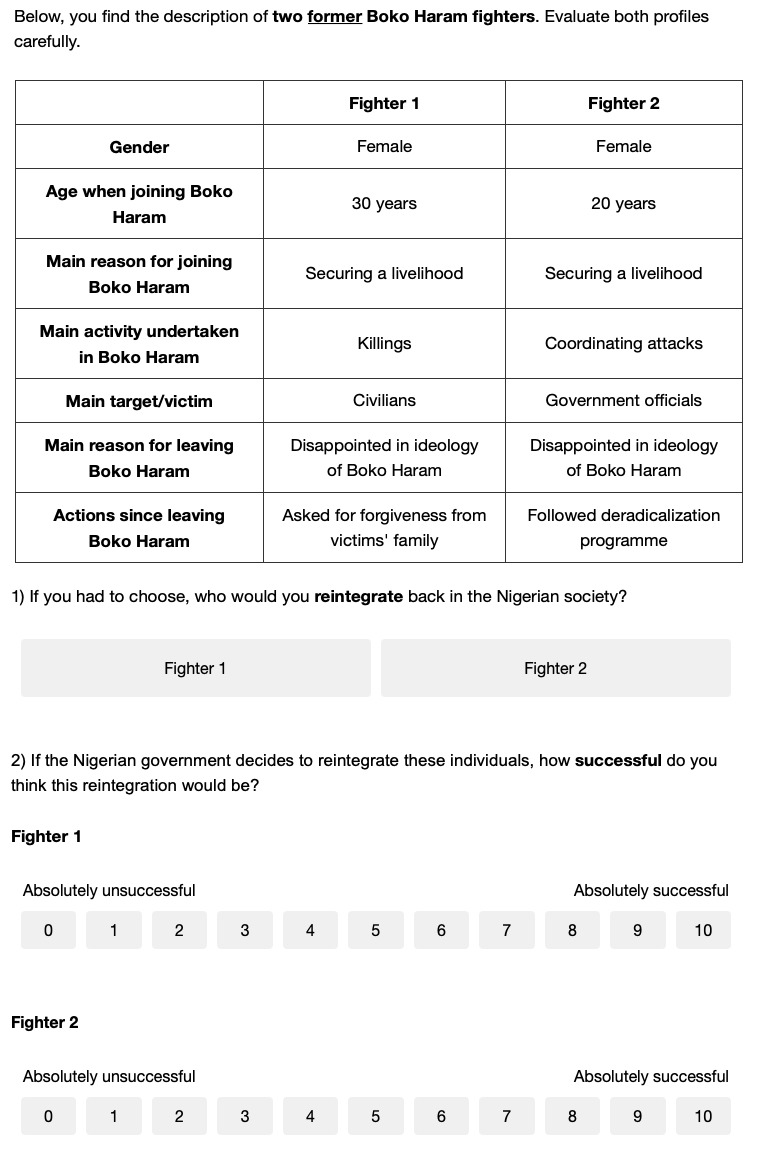
\includegraphics[height=\textheight]{Chapter_3/art2-figure1.jpg}}
\caption{Example of the Conjoint Experimental Design}
\label{fig:art2-fig1}    
\end{figure}
%----------------------------------------------------------


%---------------------------------------------------------- 
\subsection{Outcome Measures}
%---------------------------------------------------------- 

Previous research suggests that general support for counter-terrorism policies might be driven by reasons other than perceptions of effectiveness \citep{Clubb2019}. We therefore asked two questions as dependent variables (see Figure \ref{fig:art2-fig1}). First, respondents were asked to choose which ex-fighter they preferred to reintegrate back into the Nigerian society. This represents a `forced-choice' design which enables us to ``evaluate the role of each attribute value in the assessment of one profile relative to another'' \citep[][p. 4]{Hainmueller2014a}. Second, respondents indicated how successful they thought the reintegration of both ex-fighters would be. Such a `rating-based' design enables evaluations of success for each fighter separately and allow us to calculate the overall belief in the process of reintegration. Because the effects of all attribute features are measured on the same two scales, the importance of each attribute feature can be directly compared \cite[][but see Leeper et al., 2019]{Hainmueller2014a}.


%---------------------------------------------------------- 
\subsection{Estimation and Interpretation}
%---------------------------------------------------------- 

The two most popular quantities of interest to estimate when using a conjoint experiment are \textit{average marginal component effects} \citep[AMCEs;][]{Hainmueller2014a} and \textit{marginal means} \citep[MMs][]{Leeper2019}. While AMCEs have a \textit{causal }interpretation (i.e., the degree to which a certain attribute level increases or decreases the observed selection probability or favorability relative to the baseline), MMs have a more \textit{descriptive }interpretation (i.e., the observed selection probability or favorability towards a given feature over alternative values of each feature).\footnote{Two things are worth highlighting here. First, AMCEs are defined given a set of baseline attributes. In our analyses, the least-liked former fighter represents the baseline. Second, we follow \cite{Abramson2019} in interpreting MMs as \textit{revealed} preferences or \textit{observed} choices made in the experiment and not as underlying true preferences of the majority. See Appendix \ref{app:C21} for more information on the quantities of interests and their interpretation.} This difference between AMCEs and MMs becomes especially important when testing heterogeneous treatment effects because interactions using categorical variables are sensitive to the reference category used in the analysis. When the subgroups differ in their preference vis-a-vis the reference category, differences in AMCEs can be incorrectly interpreted as differences in subgroup preferences \citep{Leeper2019}. Hence, below, we report AMCEs and MMs when estimating main effects, but only conditional MMs when estimating heterogeneous treatment effects. To estimate all AMCEs and MMs, we used the \textit{cregg} package in R \citep{Leeper2018a}. Importantly, we account for the conditionally independent randomization by calculating quantities of interest over the completely observable portion of the feature of interest \citep{Leeper2019}.\footnote{ More specifically, we calculate the quantities of interest over (1) the levels of the feature of interest only, (2) subsets of the design that are conditionally unconstrained, and (3) all features with the explicit caveat that the comparison happens across dissimilar subsets of profiles for the age, gender, atrocity, and victim attributes. Overall, although there are some minor discrepancies, the restrictions do not substantially alter the results. Results from model (1) are reported in this chapter. See Appendix \ref{app:C22} for the exact equations estimated and numerical results from all models.}


%---------------------------------------------------------- 
\section{Results}
%---------------------------------------------------------- 
In this section, we present the experimental results in three parts. First, we evaluate the impact of ex-fighter characteristics on the selection probabilities using the forced-based outcome question. Second, we evaluate the impact of the same characteristics on civilian perceptions of the successfulness of reintegration using the rating-based questions. Last, we probe for heterogeneous treatment effects based on the religious background of our respondents, their exposure to Boko Haram violence, and their self-reported anger reactions to this violence.


%---------------------------------------------------------- 
\subsection{Impact of Characteristics of the Former Fighters on Selection}
%---------------------------------------------------------- 

\subsubsection{Gender and Age}
The results yield little evidence that respondents differentiated between having to reintegrate a male or female ex-fighter. The point estimate suggests that female ex-fighters are only slightly (i.e., 2.65\%) more likely to be chosen, though this effect still falls within the conventional levels of statistical significance ($p = .004$, all \textit{p}-values reported are from two-tailed tests). In contrast, our findings indicate that the age at which the fighter joined the insurgency is an important driver of citizens' reintegration attitudes. As Figure \ref{fig:art2-fig2} below shows, the probability to be selected for reintegration decreases more or less monotonically with the age at which someone decided to join the insurgency. For example, a Boko Haram fighter who was born within the insurgency is 15.11\% more likely to be selected for reintegration compared to fighter who joined the insurgency at age 30 ($p < .001$).\footnote{Results from the full model reported in Appendix \ref{app:C22} slightly divert from these results, especially for those fighters born within the Boko Haram insurgency. However, the estimates for the attribute Age in the full model in \ref{app:C22} should be interpreted with caution as fighters born within Boko Haram could display no other reason to join the insurgency but to be forced. Hence, these estimates are averaged over a different set of feature combinations. The results reported in the chapter are averaged over a comparable subset of feature combinations.}


\subsubsection{Motivation, Atrocity, and Target of Violence}
In keeping with the results of age, combatants who were forced to join Boko Haram are more likely to be chosen compared to fighters who joined Boko Haram for any other reason. More specifically, 60.76\% of the time respondents selected an ex-combatant who was forced to join the insurgency. Joining Boko Haram for the establishment of a Caliphate is especially detrimental since all other reasons significantly increase the probability of selection (all $p < .001$). Surprisingly, the specific atrocities committed while enrolled in Boko Haram do not play a substantial role in affecting reintegration attitudes. The marginal means for the specific atrocities range from 46.35 for rape to 53.31 for kidnappings. Compared to rape, kidnappings (AMCE = 0.07, $p = .001$) and the coordination of attacks (AMCE = 0.05, $p = .02$) slightly, but significantly, increase the probability to be selected. In addition, the target of those atrocities do not substantially impact attitudes towards reintegration either, although targeting Christians produces a small decrease the probability of selection compared to all other possible targets included in the experiment (all $p < .063$).


\subsubsection{Abandonment and Reconciliation}
The results further reveal that the two features concerning the aftermath of involvement in Boko Haram display some of the largest effects on the probability that a former fighter is chosen to be reintegrated. First, the reason why someone left the insurgency substantially affects citizens' willingness to reintegrate this former fighter. Fighters abandoning Boko Haram out of remorse for their violent behavior or disappointment in the ideology of Boko Haram are most likely to be chosen (i.e., 61.59\% and 58.17\%, respectively), whereas being injured and hospitalized or captured by the military display the lowest marginal mean (i.e., 42.89\% and 41.37\%, respectively). Fighters who quit the insurgency because they were uncertain about the survival of Boko Haram are selected 46.04\% of the time. Second, post-conflict reparations are also key to reintegration attitudes. More specifically, helping the police and military to combat Boko Haram increases the probability of selection with 23.84\% compared to doing nothing ($p <.001$). The distributive (i.e., paying a fine) and two restorative justice provisions (i.e., asking forgiveness and offering apologies) produce a roughly 12\% and 14\% increase in the probability that an ex-fighter is selected compared to the baseline of no reparations (all \textit{p}'s $\mathrm{<}$ .001). Following a deradicalization program also positively impacts reintegration attitudes as it increases the probability of selection with 14.30\% ($p < .001$). Interestingly, there does not seem to be much difference in selection probabilities between ex-Boko Haram members who provide monetary reparation, who apologize or ask forgiveness, or those who followed a deradicalization program.


%----------------------------------------------------------
% Figure 2
%----------------------------------------------------------
\begin{figure}[H]
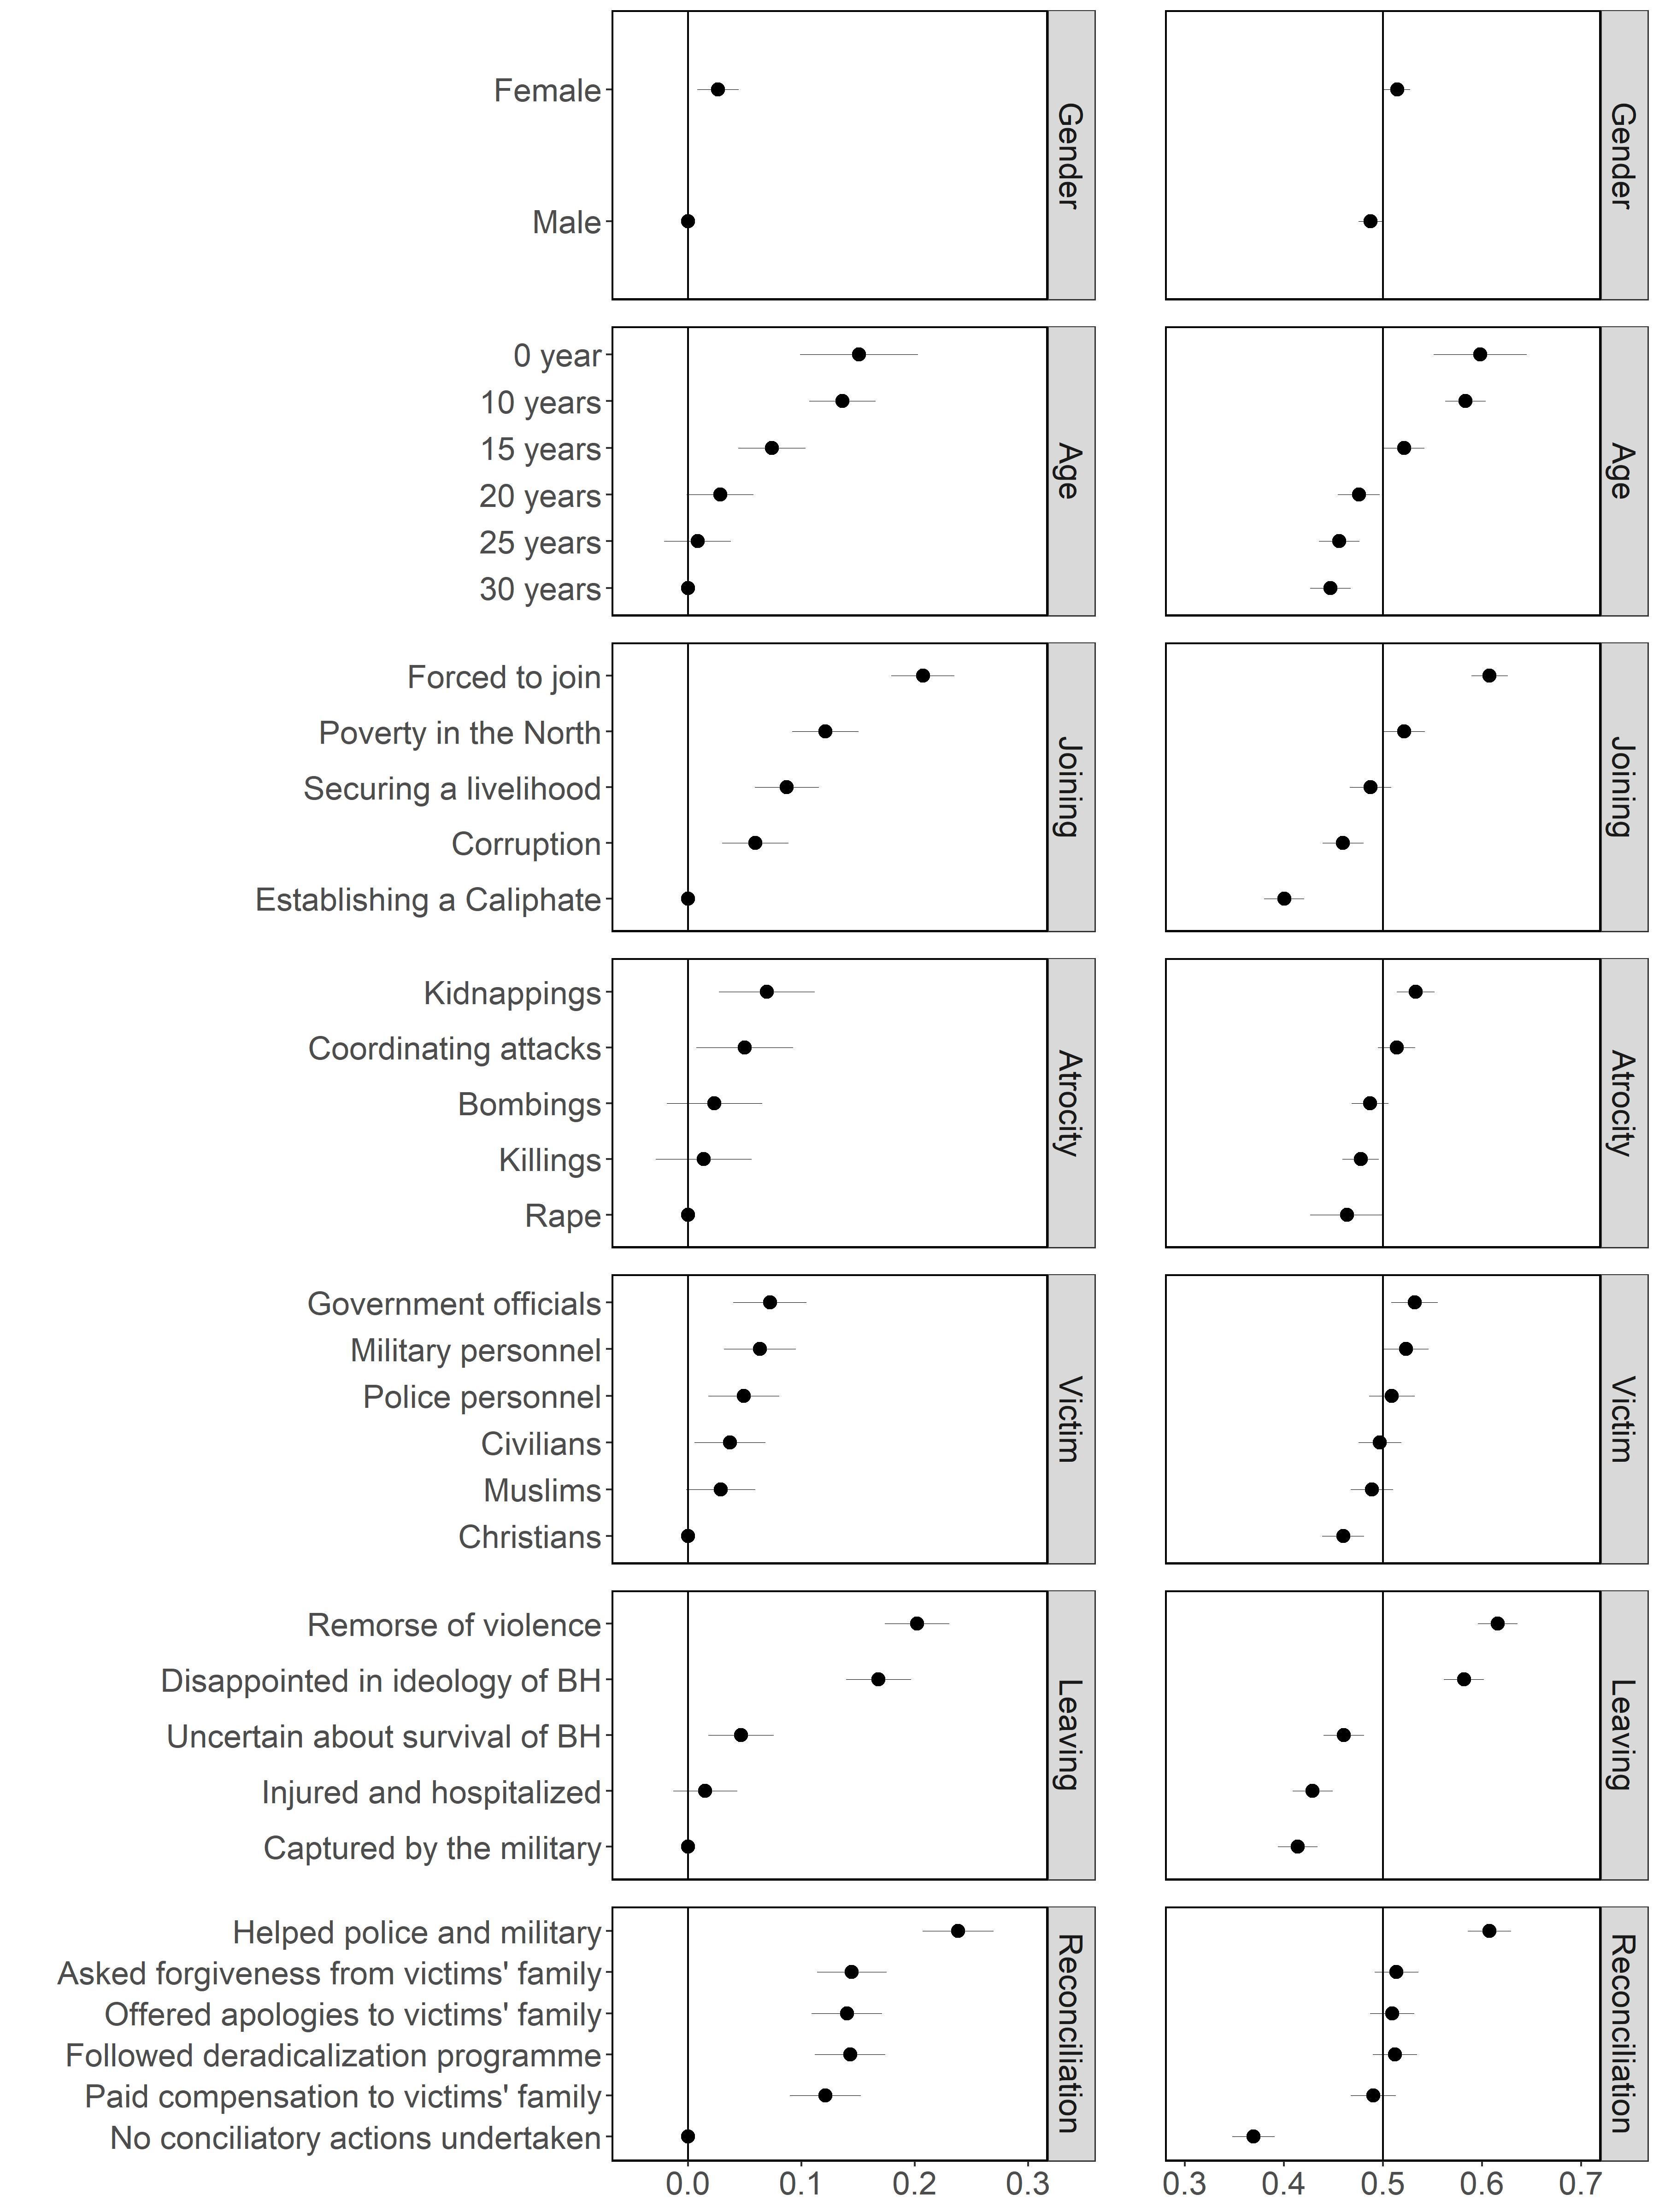
\includegraphics[width=\textwidth]{Chapter_3/art2-figure2.jpeg}
\caption{Estimated Average Marginal Component Effects (Left) and Marginal Means (Right) for Choice-Based Design}
\label{fig:art2-fig2}    
\end{figure}
%----------------------------------------------------------

%---------------------------------------------------------- 
\newpage
\subsection{Impact of Characteristics of the Former Fighters on Success}
%---------------------------------------------------------- 

Next, we are interested in the determinants shaping perceptions of success of reintegration. In general, there is quite some uncertainty about the success of reintegration given that the overall mean circles around the midpoint of the scale ($M = 5.45$, $SD = 2.41$).\footnote{An empty random intercept multilevel model, with ratings clustered within respondents, confirms that $\beta_0 = 5.45$ ($S.E.=0.039$).} Furthermore, as Figure \ref{fig:art2-fig3} below shows, the estimates largely mimic the results from the forced-based design which adds robustness to our findings. Respondents have more faith in the reintegration process of ex-fighters who were forced to join, who showed remorse of violence or disappointment with the ideology of Boko Haram, or who helped the police and military to combat Boko. Any other distributive or restorative justice mechanism also increases success perceptions (all \textit{p'}s\textit{ }$\mathrm{<} .001$). In contrast, our participants are more skeptical about welcoming back ex-combatants who joined the insurgency out of religious beliefs, were captured by the military or injured and hospitalized, or showed no sign of reconciliation. Information related to the ex-fighters' gender, age when joining the insurgency, committed atrocities, or targeted victims do not substantially change perceptions of success.\footnote{It is worth noting that the age at which an ex-combatant joined the Boko Haram insurgency is the only variable were the results change considerably (i.e., the linear trend disappears when looking at successfulness ratings). This suggests that, when forced to choose one fighter to reintegrate, respondents feel to some extent obliged to select younger fighters who are less responsible for their acts. When they have to rate the success of reintegration, however, respondents acknowledge young fighters, especially those born within Boko Haram, will equally face serious challenges during their reintegration stage.} 

As suggested by \cite{Johns2019}, these results constitute a key first step in identifying \textit{potential} mechanisms through which ex-combatants' characteristics influence reintegration attitudes. Similar to \cite{Johns2019}, we stress the word \textit{potential} because our design did not permit an unbiased mediation analysis given that perceptions of success were measured post-treatment instead of manipulated explicitly and separately \citep{Bullock2011}. Yet, given that our rating-based results show roughly the same pattern of effects as on the choice-based variable, perceptions of success hold the potential to act as a mechanism stimulating willingness to reintegrate certain ex-fighters.

%----------------------------------------------------------
% Figure 3
%----------------------------------------------------------
\vspace{3mm}
\begin{figure}[H]
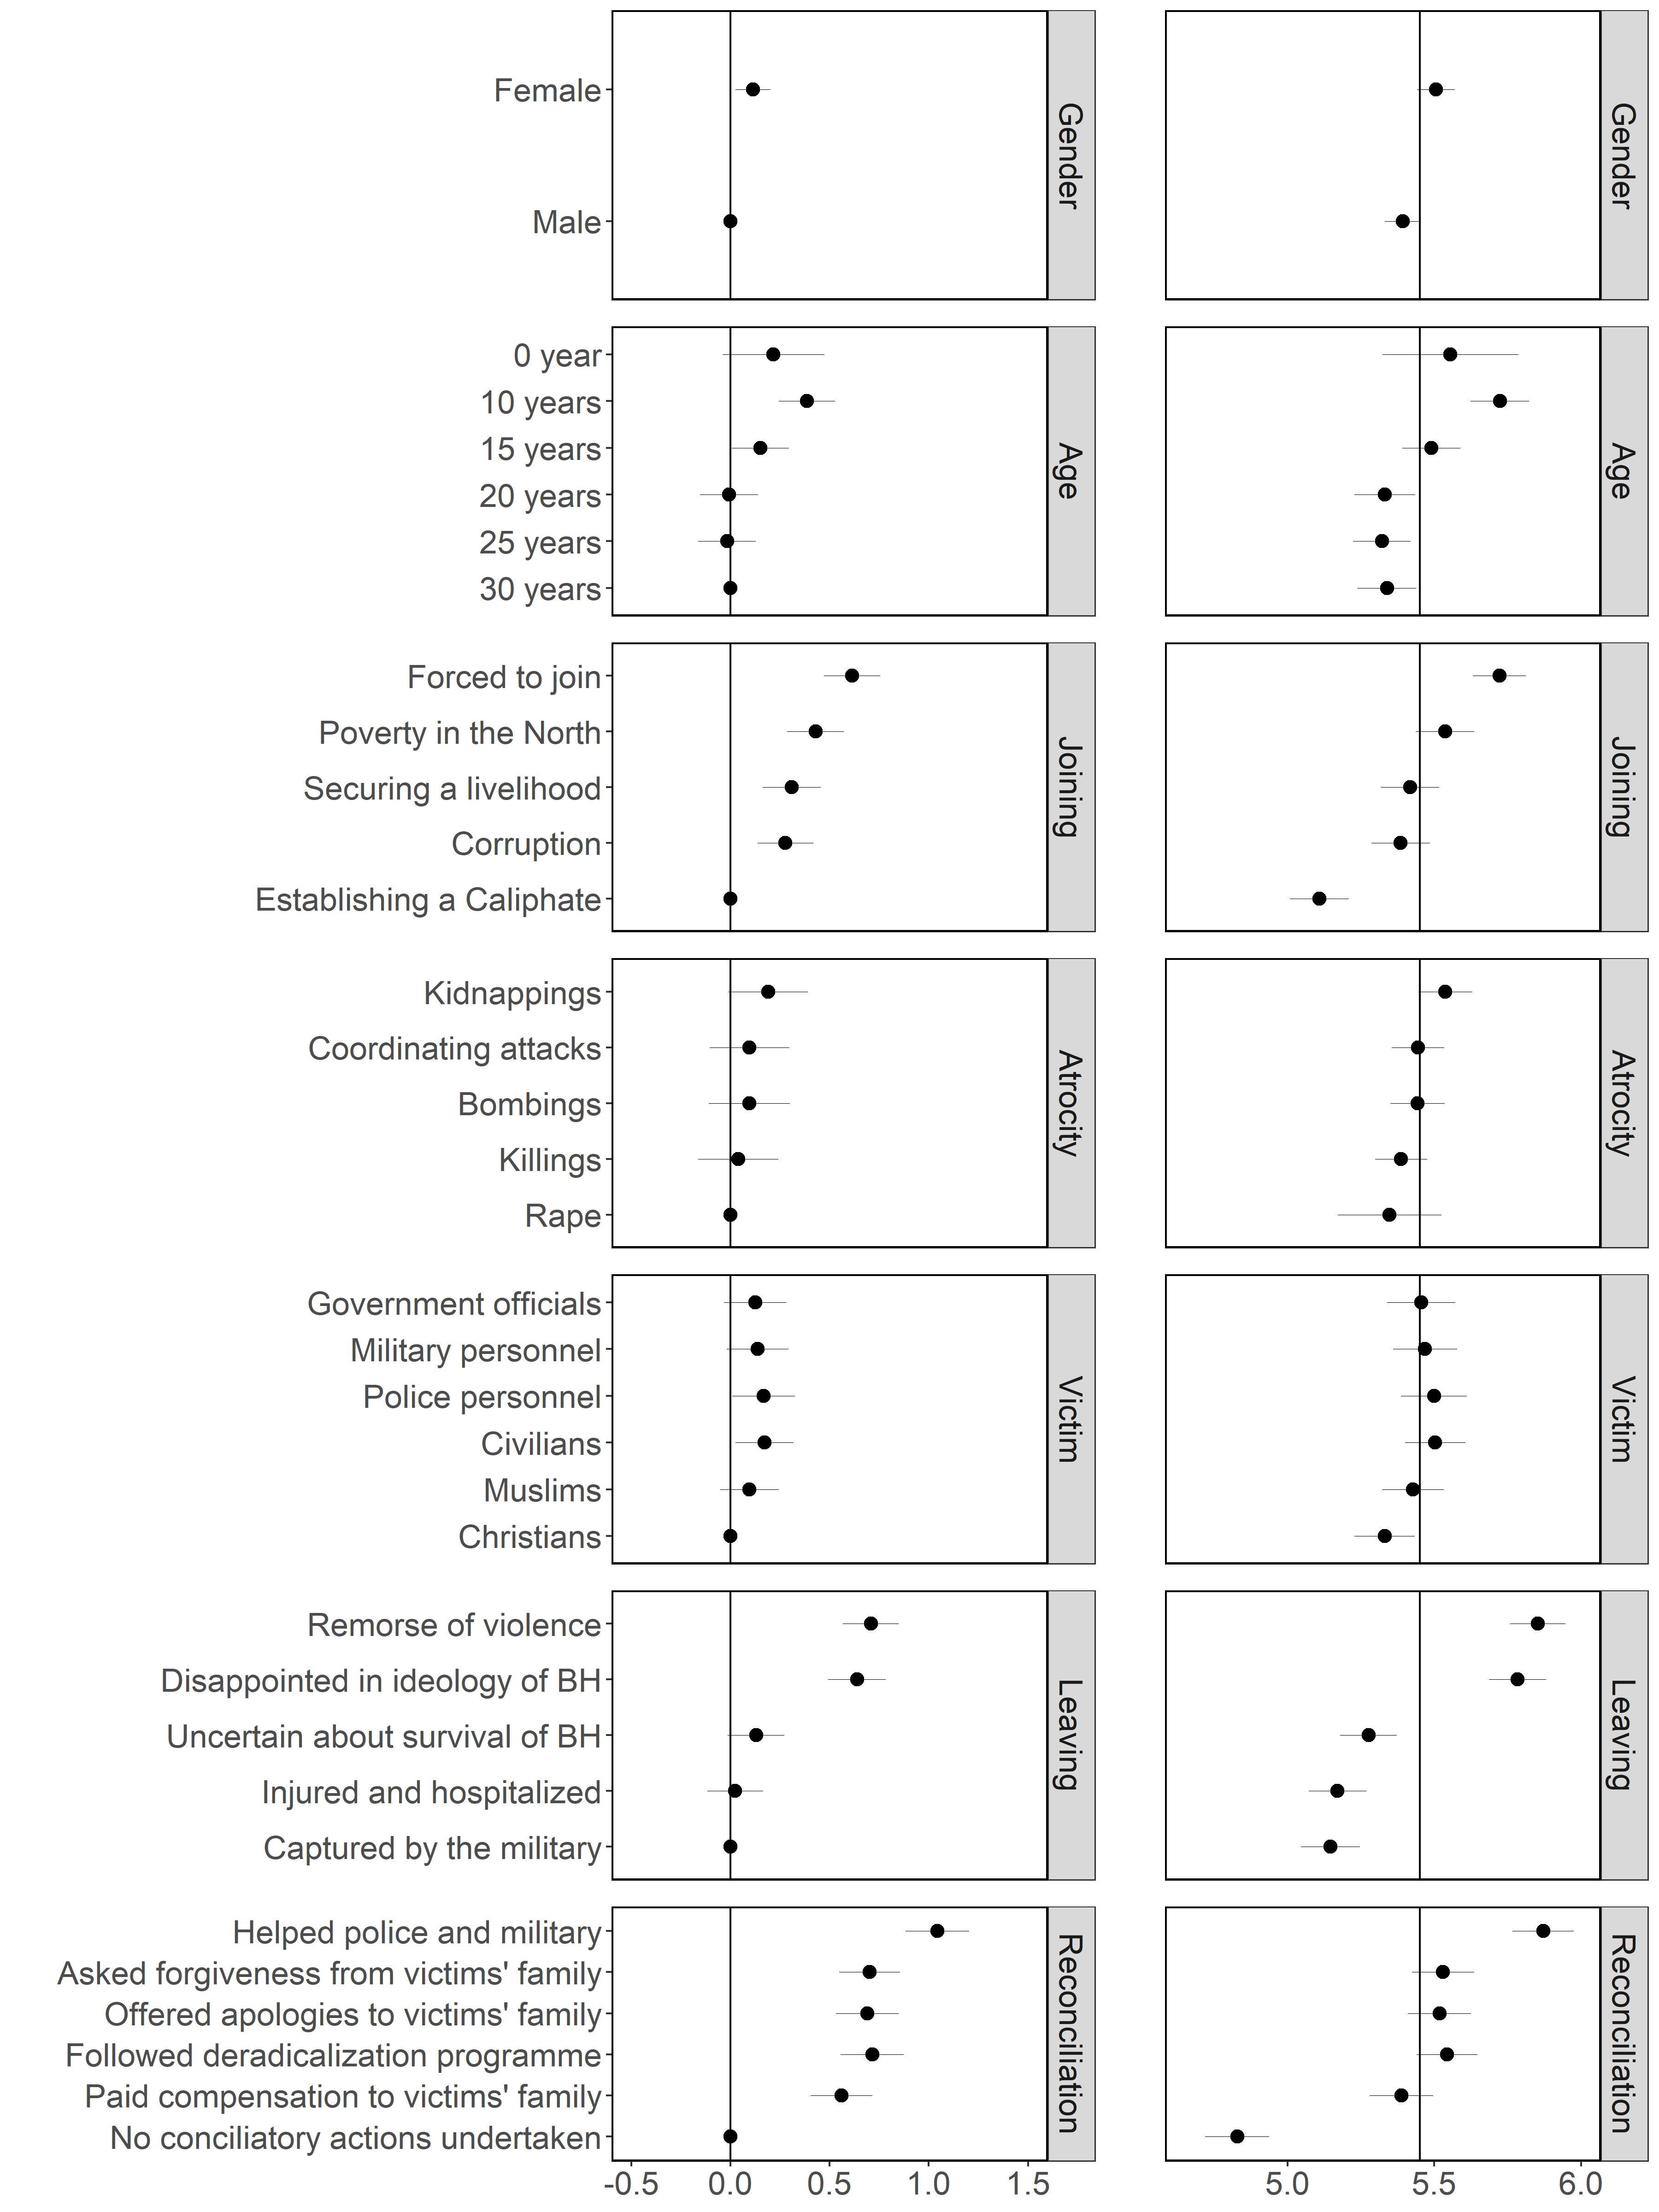
\includegraphics[width=\textwidth]{Chapter_3/art2-figure3.jpeg}
\caption{Estimated Average Marginal Component Effects (Left) and Marginal Means (Right) for Rating-Based Design}
\label{fig:art2-fig3}    
\end{figure}
%----------------------------------------------------------

%----------------------------------------------------------
\newpage
\subsection{Moderating Impact of Respondent Characteristics }
%----------------------------------------------------------
The public itself might equally vary in its preferences for reintegration along important conflict-related characteristics. To address the question of whether characteristics of the respondents moderate the effects of the treatment, we estimate a series of models interacting the treatment with each of these respondent traits. Specifically, six models are fitted as we test three moderators (i.e., respondents' religion, exposure to Boko Haram violence, and anger reactions to the violence) on both the choice-based and rating-based outcome variable. All conditional MMs are displayed in Figure \ref{fig:art2-fig4}, \ref{fig:art2-fig5}, and \ref{fig:art2-fig6} below, while we now briefly elaborate on the most important results.

The religious background of the respondents interacted, to a small extent, with the treatment. First, Christians and Muslims slightly differed in the importance attached to transitional justice provisions when choosing which fighter they want to reintegrate back into the Nigerian society (\textit{F} = 2.31, \textit{p} = .03).\footnote{We formally tested all subgroup differences in preferences by comparing a regression with and without interaction terms between the sub-grouping covariate and feature levels.} In particular, Christians are more suspicious of ex-combatants who have not undertaken any conciliatory action and slightly place more value on deradicalization programs compared to their Muslim counterparts. Interestingly, our respondents do not differ in their preferences based on whether the ex-combatant mainly targeted the respondent's own religious in-group or not (\textit{F} = 0.28, \textit{p} = .95). In other words, no in-group bias was found in our study. Second, and more substantially, Christians consistently rate the success of reintegration lower compared to their Muslim counterpart (\textit{M} = 5.30, \textit{SD} = 2.40 for Christians and \textit{M} = 6.00, \textit{SD} = 2.40 for Muslims; \textit{t}(3748.1) = $-12.74$, \textit{p }$\mathrm{<}$ .001).\footnote{A multivariate multilevel model with ratings clustered within respondents and religion included as a Level-2 predictor gives the same result ($b = 0.70$, $p < .001$).} So, although Christian and Muslim participants show the same response pattern when gauging the success of reintegration (e.g., they are both skeptical towards fighters who joined to insurgency to establish a Caliphate), Christians hold more negative attitudes vis-a-vis reintegration as such compared to Muslims (\textit{F }= 3.80, \textit{p} $\mathrm{<}$ .001). Last but not least, the two conflict-related variables did not significantly moderate reintegration attitudes (\textit{F} = 1.09, \textit{p }= .30 and \textit{F }= 1.17, \textit{p} = .17 for the choice-based and ration-based models conditioned on victimization, and \textit{F} = 1.24, \textit{p }= .10 and \textit{F }= 1.27, \textit{p} = .07 for the choice-based and ration-based models conditioned on self-reported anger). Hence, our results suggest that both victims and non-victims as well as angry and non-angry respondents share similar concerns and preferences regarding the reintegration of ex-Boko Haram fighters.

%----------------------------------------------------------
% Figure 4
%----------------------------------------------------------
\begin{figure}[H]
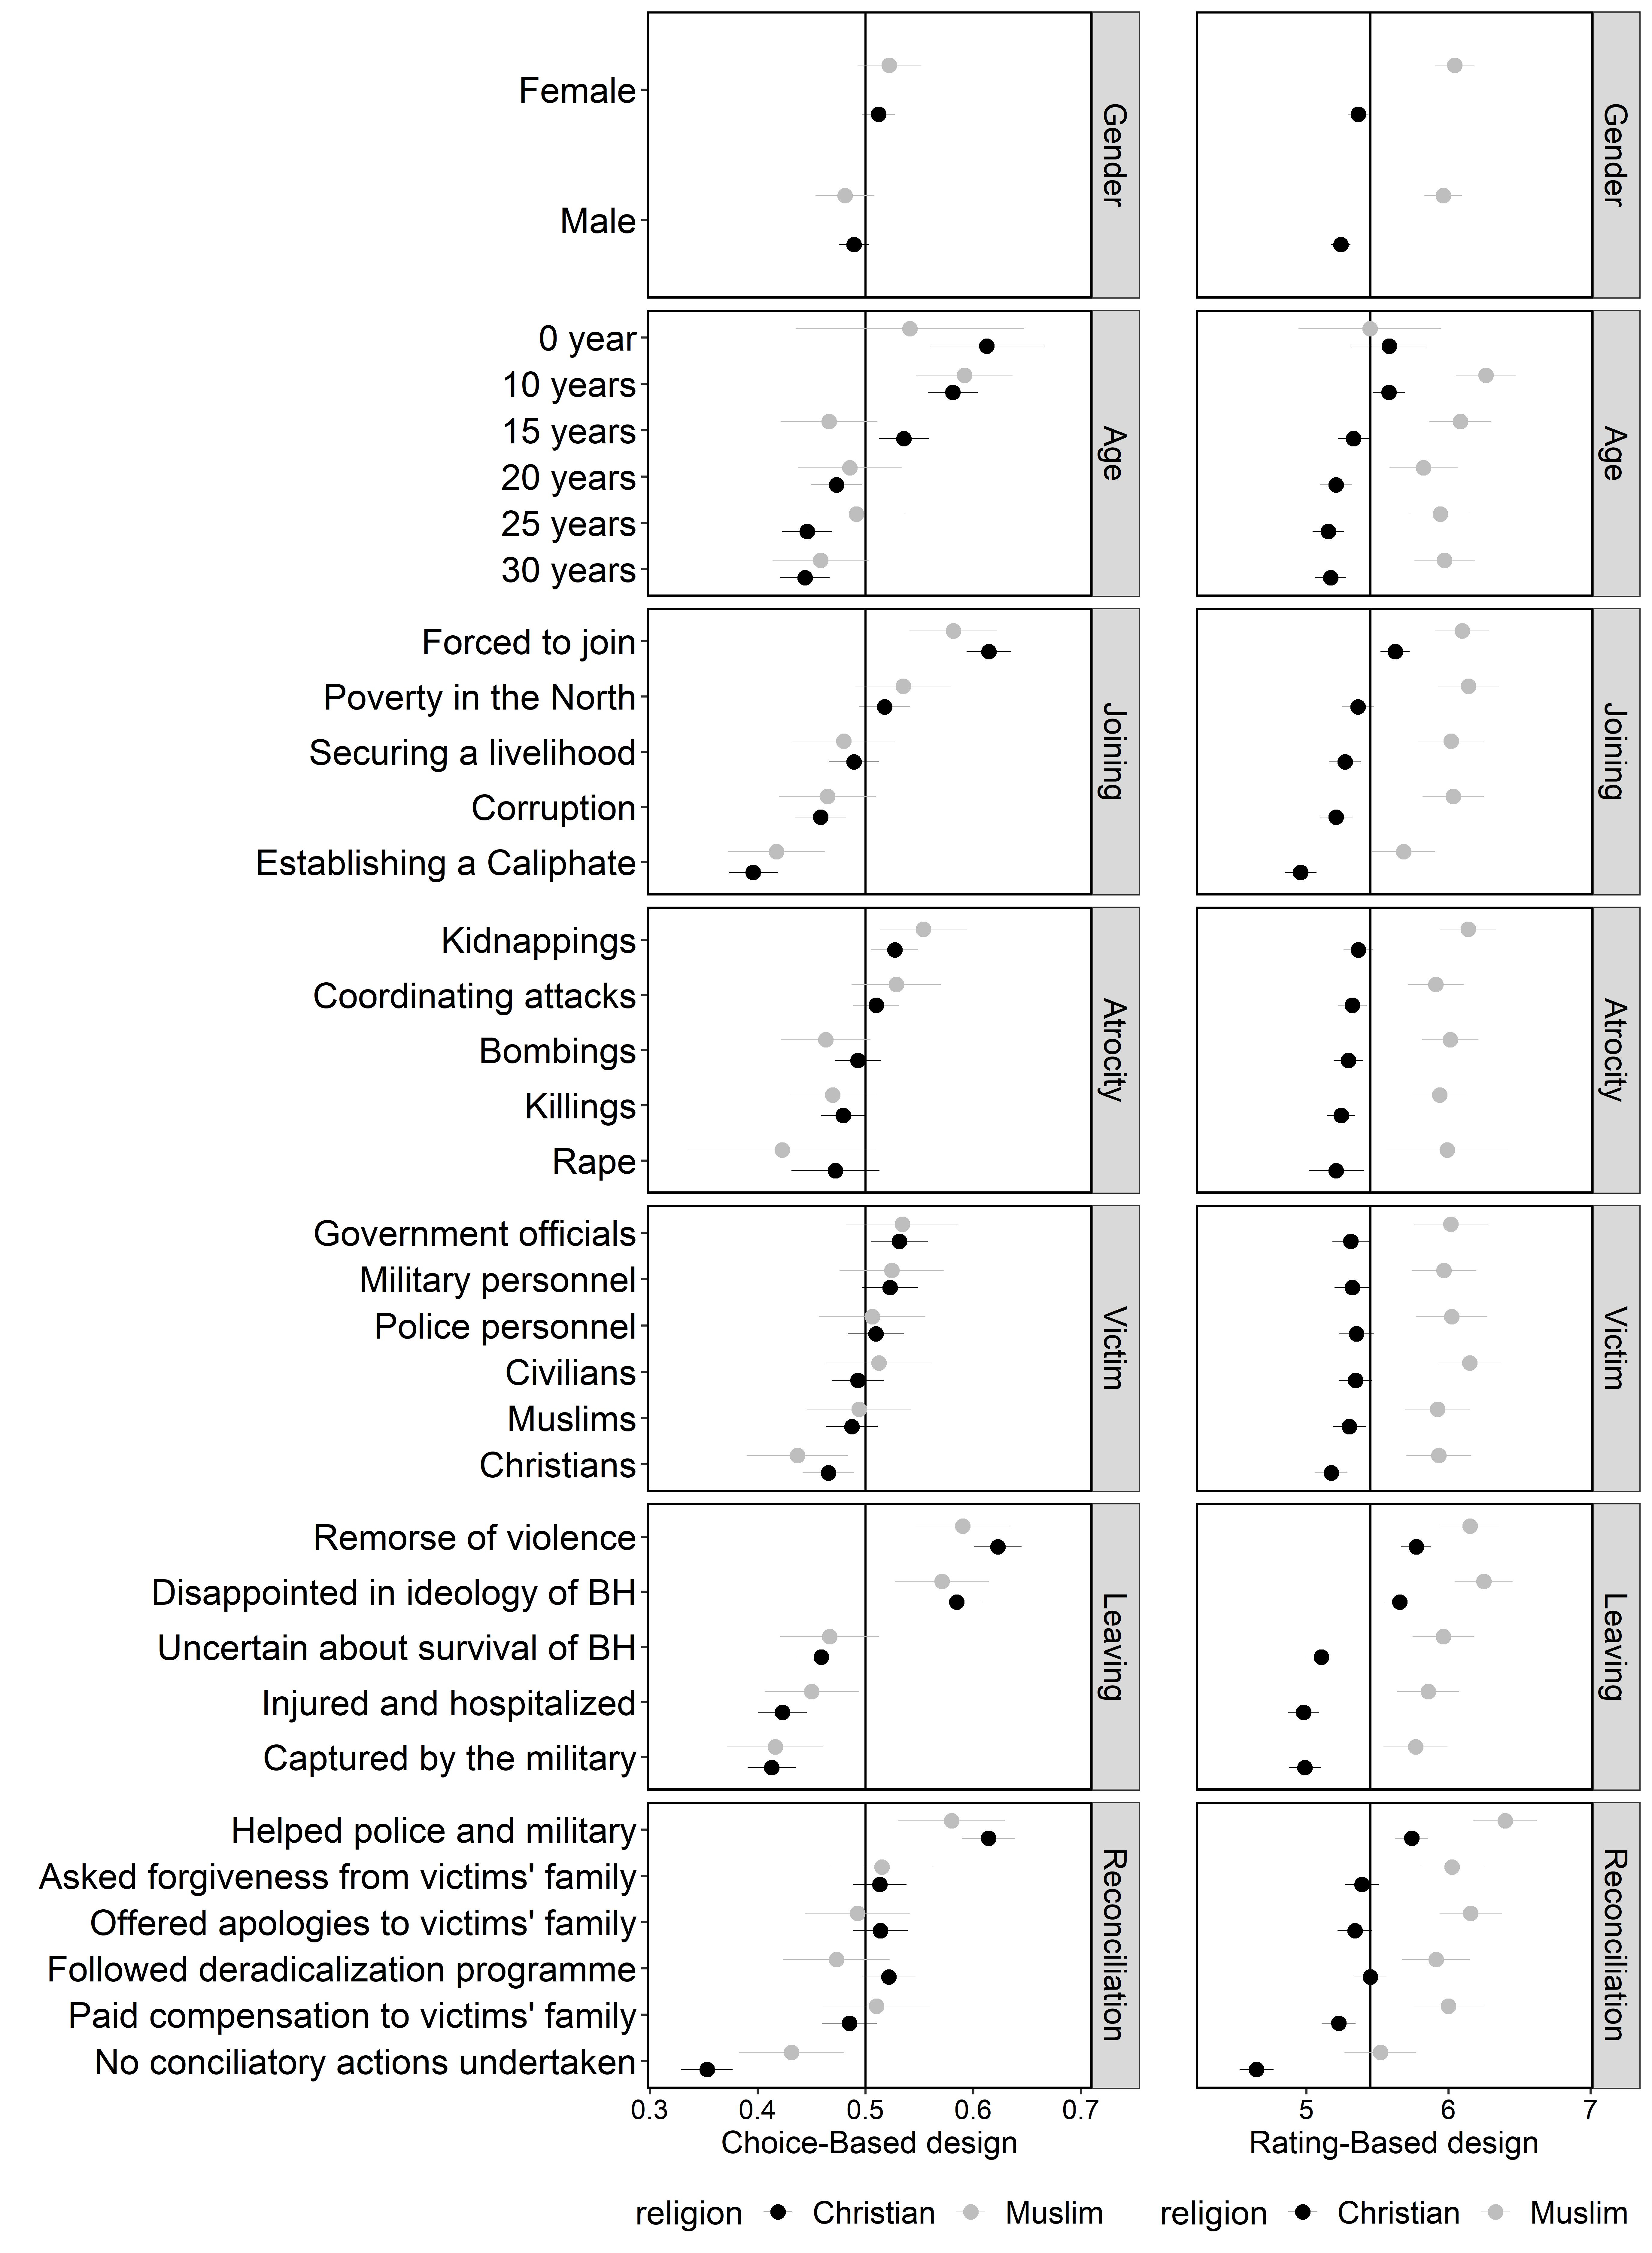
\includegraphics[width=\textwidth]{Chapter_3/art2-figure4.jpeg}
\caption{Marginal Means for Choice-Based (Left) and Rating-Based Design (Right), Conditioned on Religion}
\label{fig:art2-fig4}    
\end{figure}
%----------------------------------------------------------

%----------------------------------------------------------
% Figure 5
%----------------------------------------------------------
\begin{figure}[H]
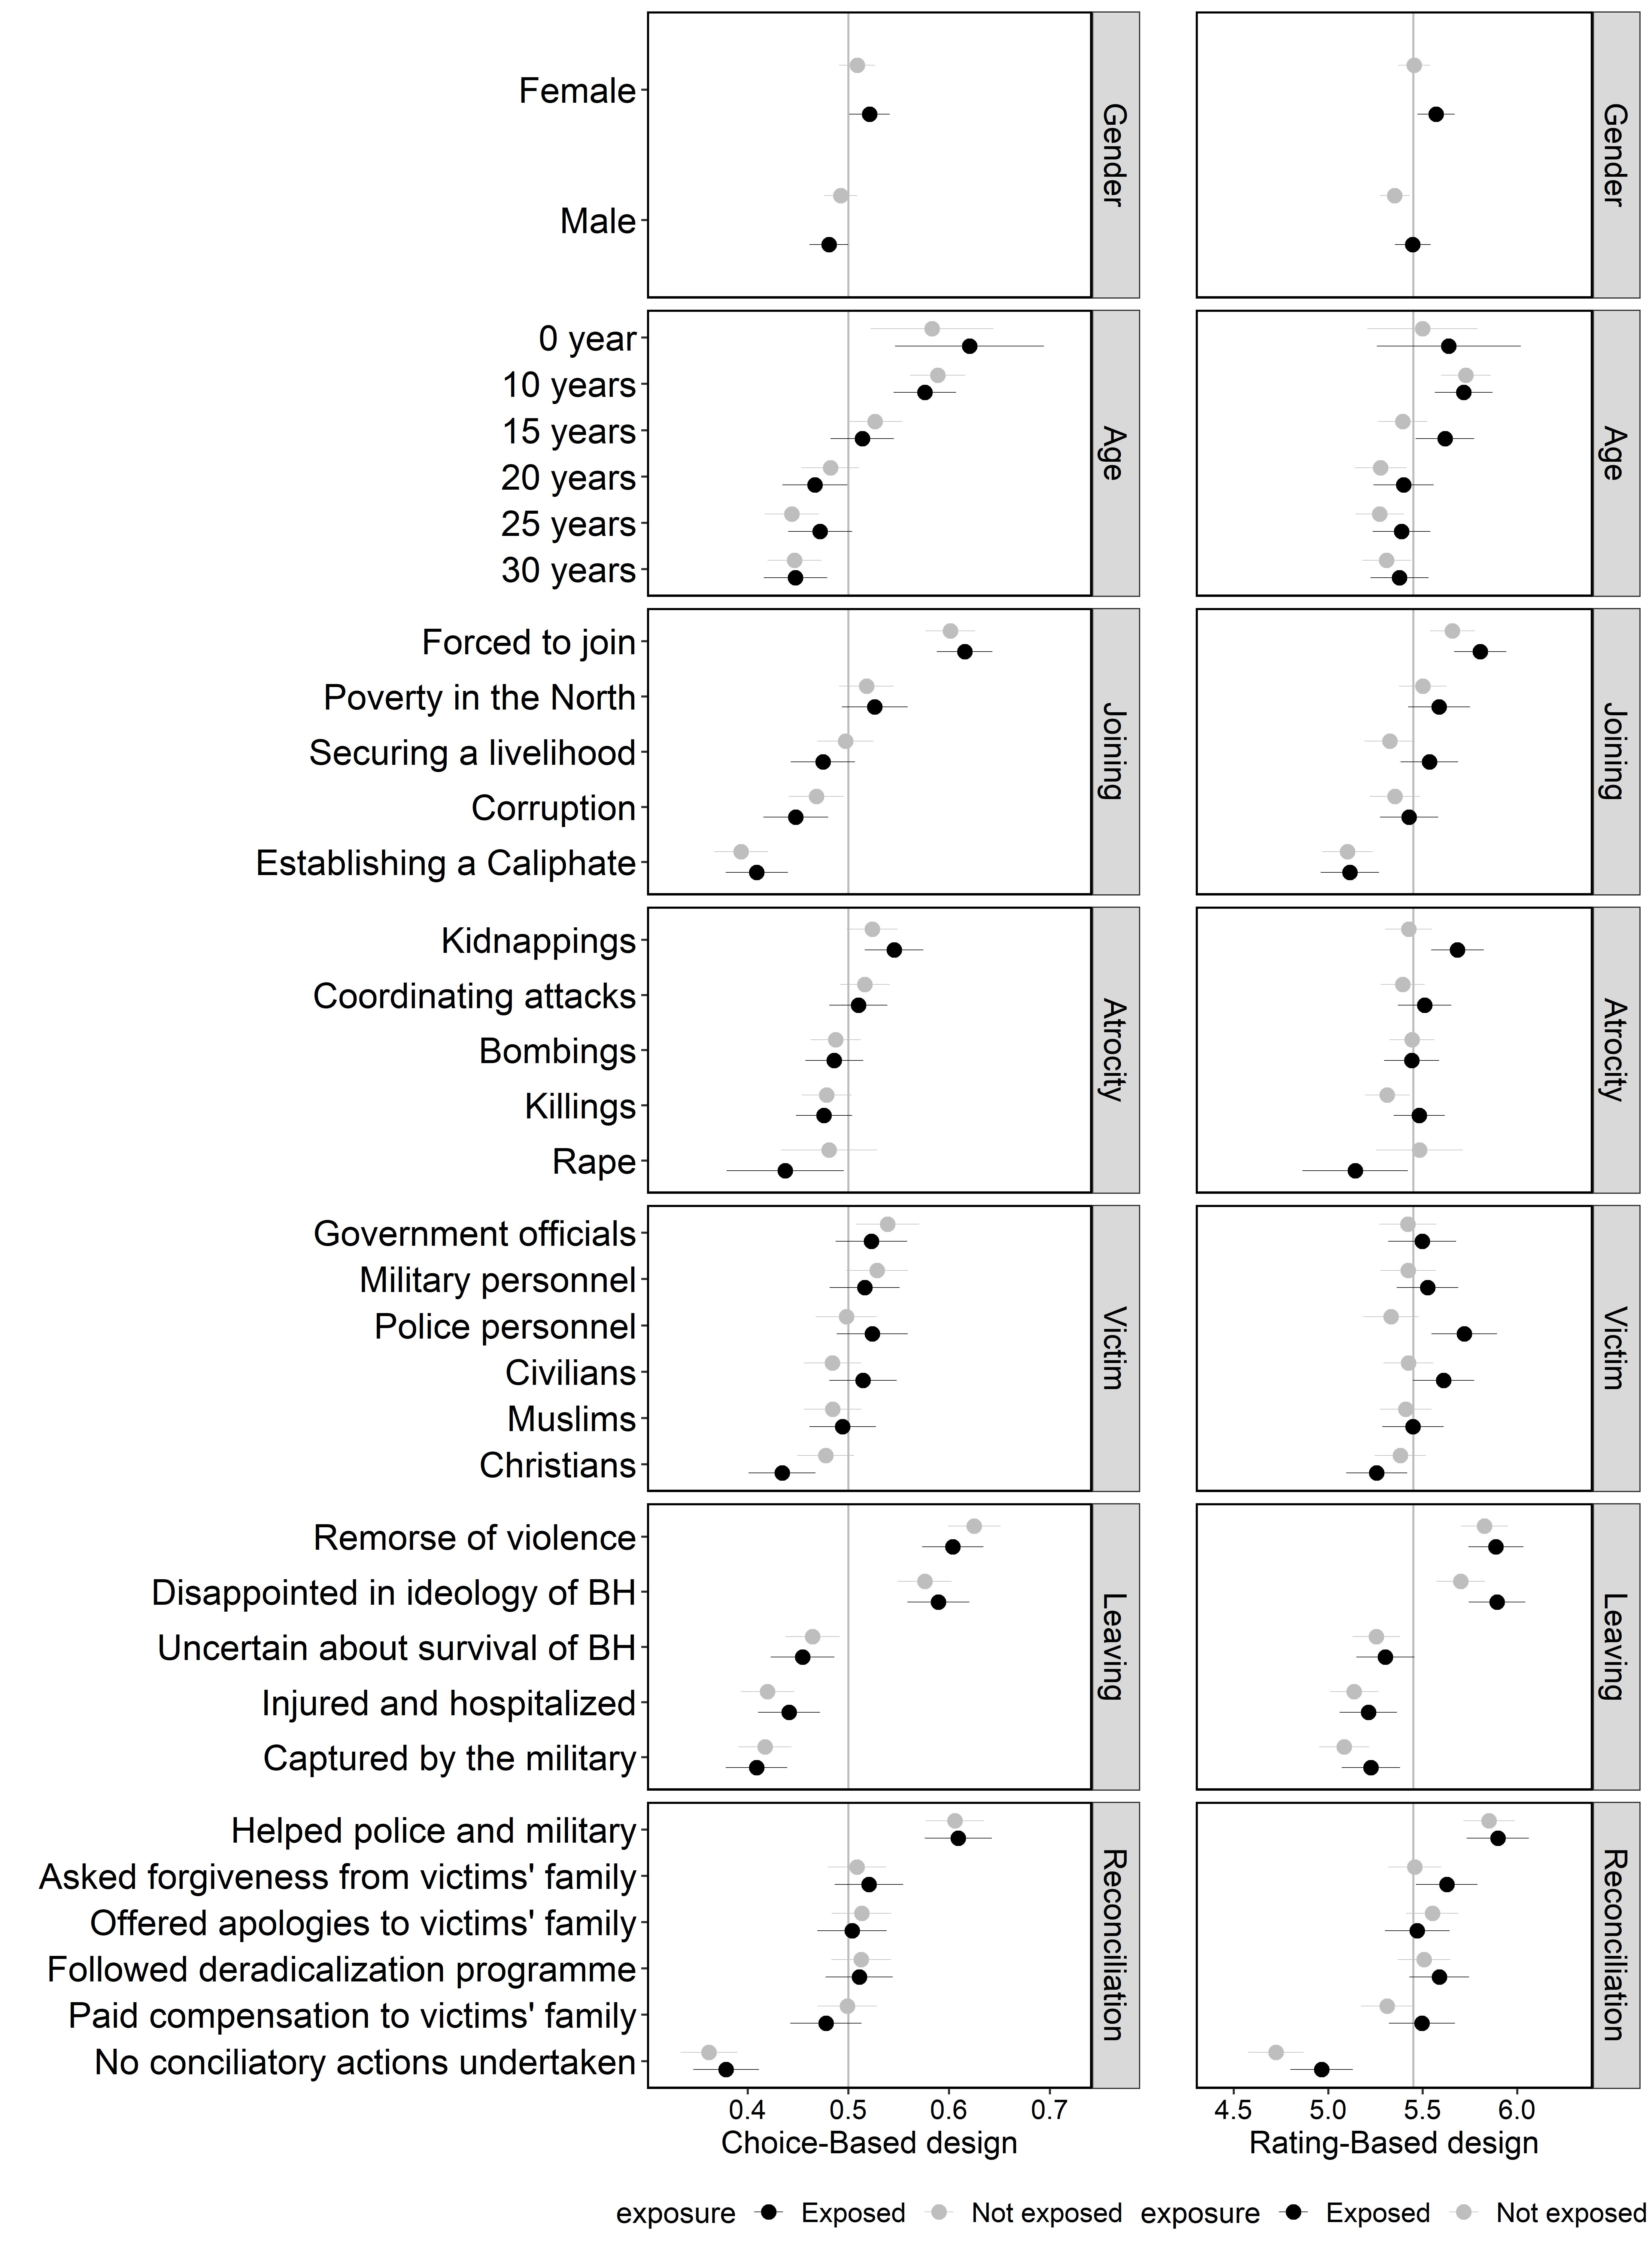
\includegraphics[width=\textwidth]{Chapter_3/art2-figure5.jpeg}
\caption{Marginal Means for Choice-Based (Left) and Rating-Based Design (Right), Conditioned on Self-Reported Exposure to Boko Haram Violence}
\label{fig:art2-fig5}    
\end{figure}
%----------------------------------------------------------


%----------------------------------------------------------
% Figure 6
%----------------------------------------------------------
\begin{figure}[H]
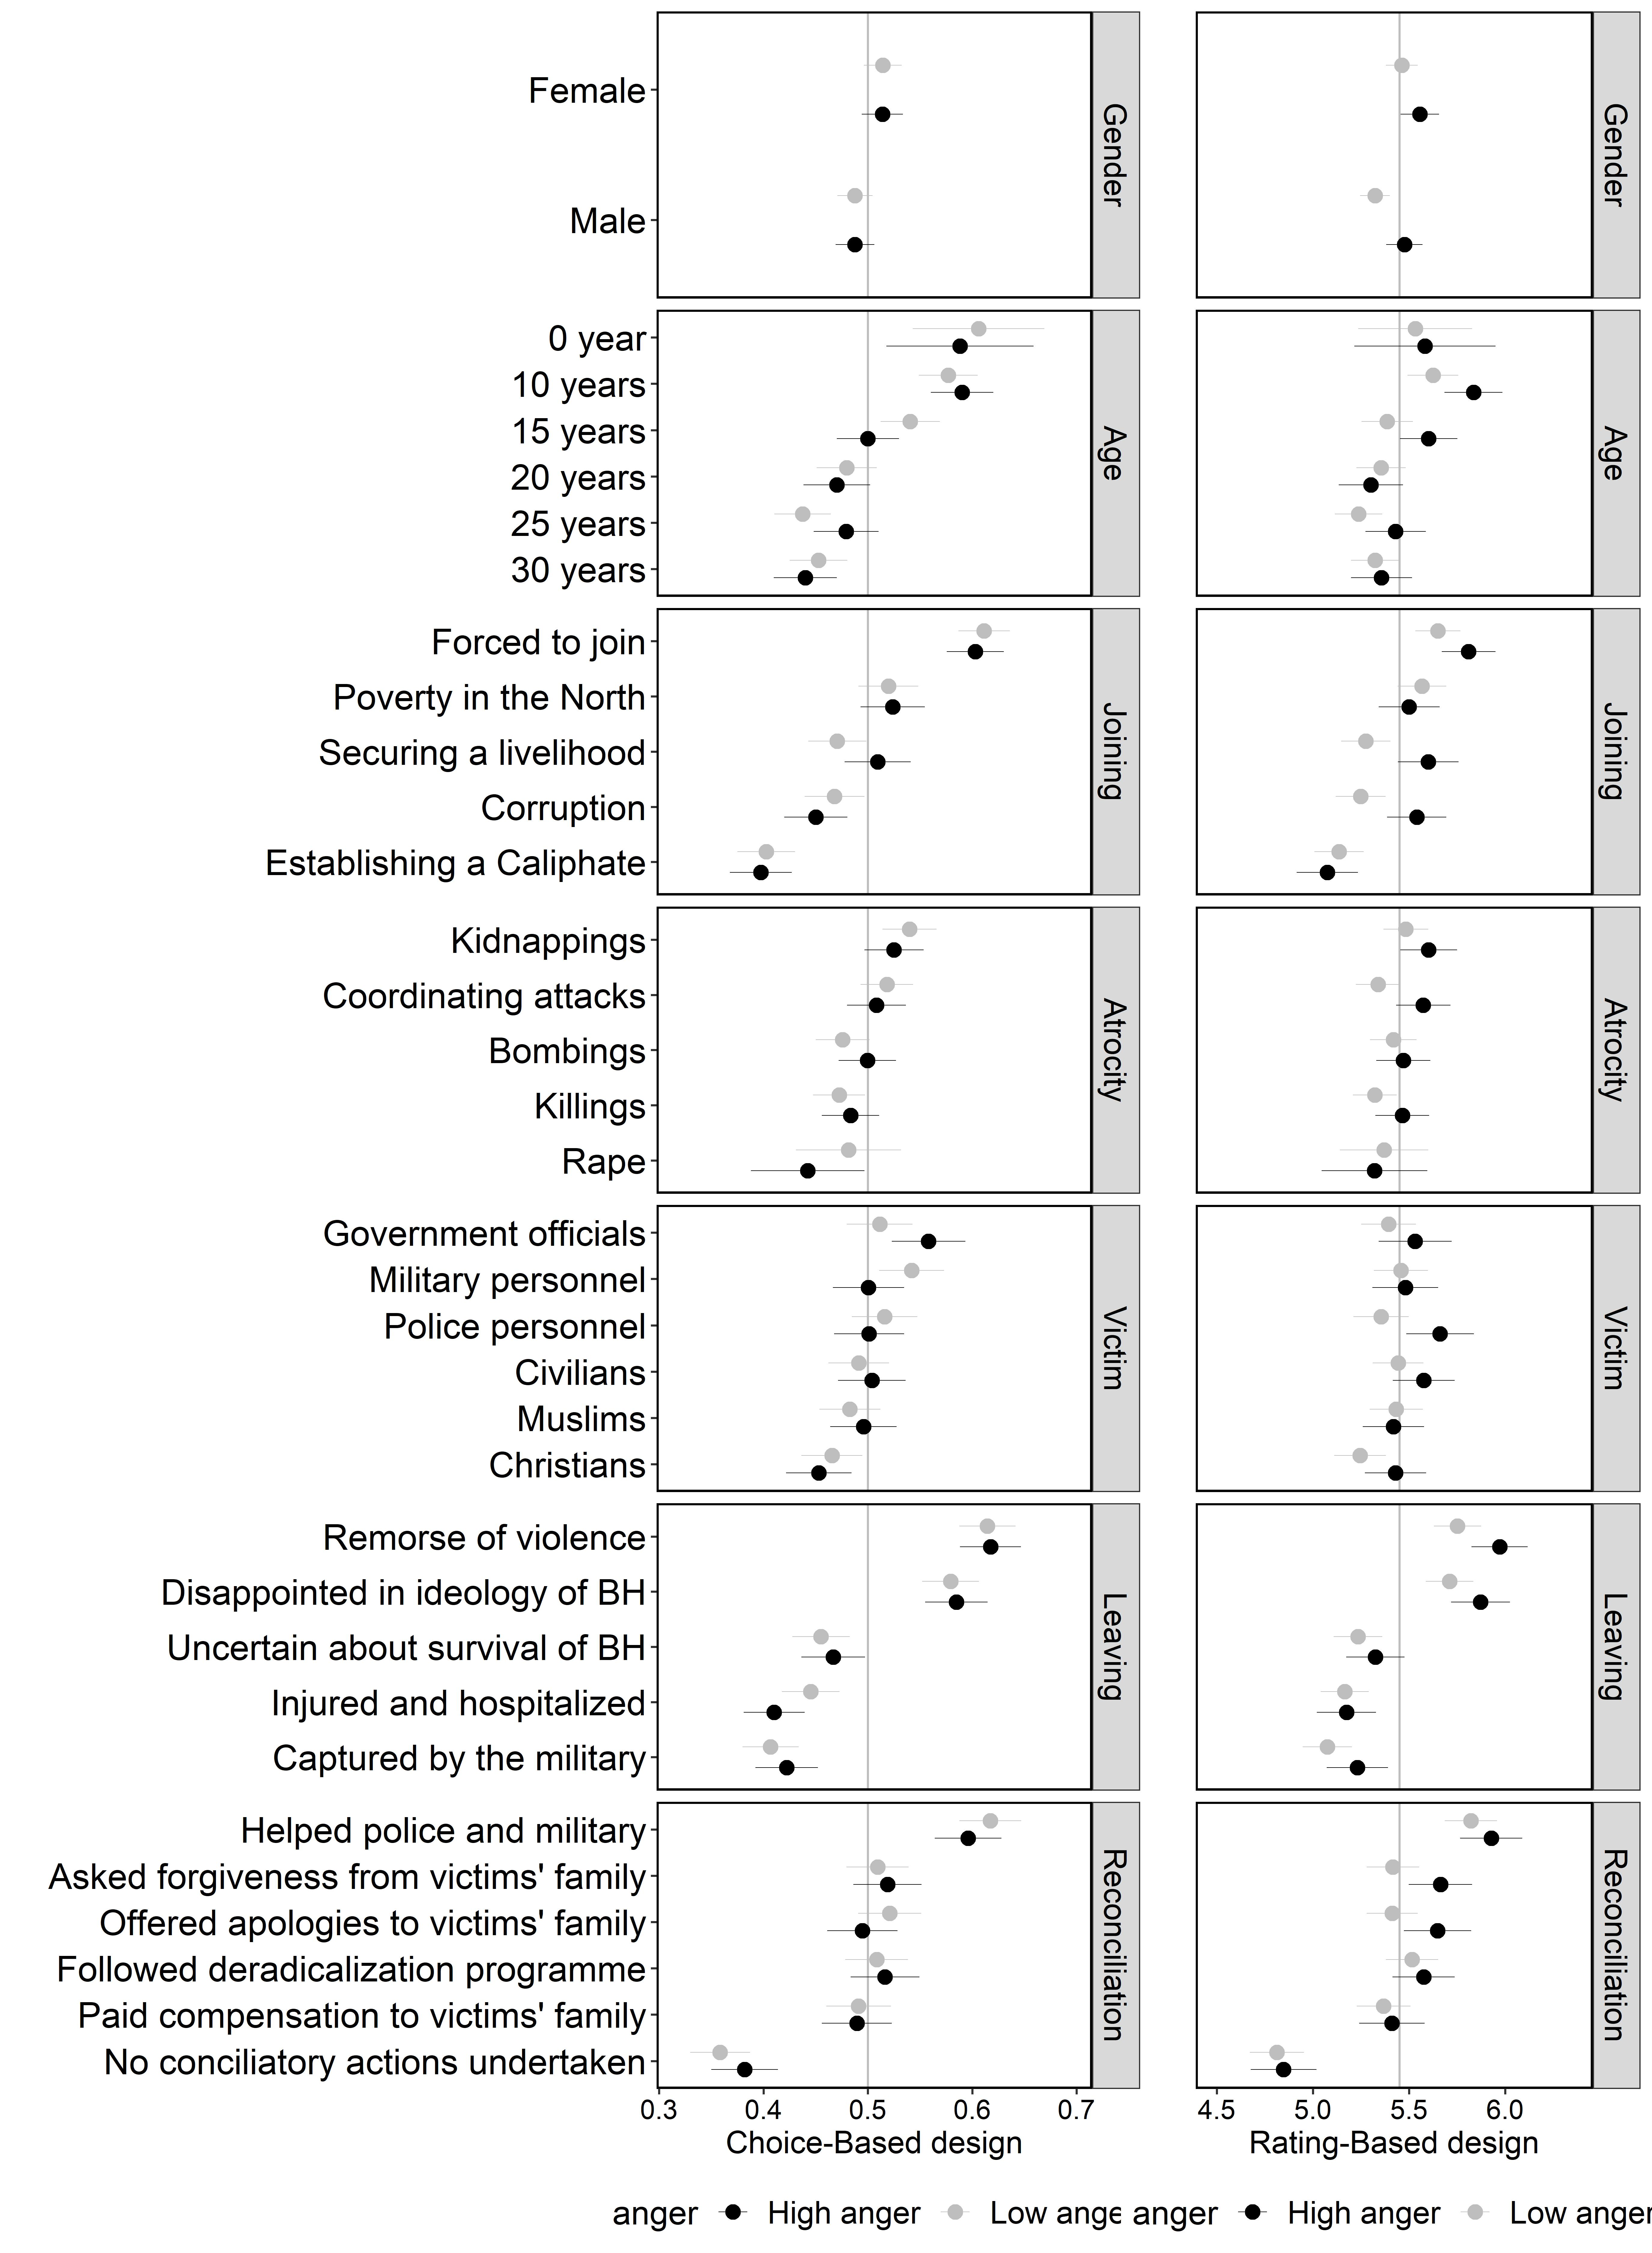
\includegraphics[width=\textwidth]{Chapter_3/art2-figure6.jpeg}
\caption{Marginal Means for Choice-Based (Left) and Rating-Based Design (Right), Conditioned on Self-Reported Anger Reactions to Boko Haram Violence}
\label{fig:art2-fig6}    
\end{figure}
%----------------------------------------------------------


%----------------------------------------------------------
\section{Conclusion}
%----------------------------------------------------------

Making peace with one's enemies is anything but easy. While conventional wisdom holds that former fighters are unwelcome ``social pariahs'' \citep[][p. 881]{Annan2011}, research on how community members think about ex-combatant reintegration is still sparse and even less has been quantitatively and/or causally identified. In this chapter, we complement previous work, which has predominantly focused on the reintegration trajectories of ex-combatants \citep[e.g.,][]{Blattman2016, Gilligan2012, UN2014}, by taking a community perspective on post-conflict reintegration. The chapter therefore speaks to the more general literature highlighting the influential role played by citizens in shaping policies \citep[e.g.,][]{Tomz2019}, including the recent work arguing that post-conflict settlements are prone to conflict recurrence when agreements fail to incorporate civilians and civil society actors \citep[e.g.,][]{Dyrstad2019, Tellez2019a}. We also contribute to the literature by employing an innovative experimental design within an understudied context. Specifically, we conducted a large-scale conjoint experiment among Nigerian young adults---a context characterized by a large-scale deradicalization and reintegration program, while simultaneously facing fierce nation-wide resistance against the reintegration of ex-Boko Haram fighters. Results from this experiment shed light on the broader debate about the reintegration of former members of violent extremist groups, which holds clear empirical, theoretical, and practical implications within and outside Nigeria.


Broadly, the empirical evidence suggests that, in a context characterized by high levels of insecurity, community acceptance of reintegration is predominantly driven by signs of remorse, repentance, and reconciliation. Indeed, for our respondents, reintegration was first and foremost dependent on being truly repentant in word and deed, as exemplified by the importance attached to former fighters leaving Boko Haram out of remorse, rejecting its ideology, helping to defeat Boko Haram in turn, and undertaking conciliatory acts. In contrast, respondents were less willing to reintegrate those fighters that exited the group because they were injured and hospitalized or captured by the military and who showed no intention to reconcile. Furthermore, information about why someone joined Boko Haram also impacted reintegration attitudes (with those forced to join being most welcome and those who joined to fight for the Caliphate least welcome), whereas information about the committed atrocity or specific target of those atrocities did not substantially alter attitudes. Our second dependent variable---that is, perceived success of reintegration---revealed that similar attributes affect belief in the process of reintegration. Although our design prohibited a full mediation analysis, these results nonetheless provide a preliminary, though important, first stage test of a potential mechanism through which ex-combatant's characteristics might influence reintegration attitudes. Last, our results showed that neither victimization nor anger reactions to violence affected opinions vis-a-vis the preconditions of post-conflict reintegration. Christians and Muslims, on the other hand, held slightly dissimilar views on the potential success of reintegration. While they both evaluated the preconditions of reintegration in similar ways, Christians were generally more suspicious about of the reintegration of ex-Boko Haram fighters. 


These findings may hold important implications for both academics theorizing about post-conflict reintegration and policymakers who must make choices about how to design and ultimately communicate reintegration programs to their public. From a theoretical perspective, taken together, our results suggest that perceptions of agency may play a crucial role in fueling belief in the process of reintegration and, ultimately, reintegration acceptance. More specifically, community acceptance of former fighters seems to be fostered by the absence of agency during the fighter's entry phase and presence of agency during his/her exit and post-exit phase. We invite future research to further explore this possible overarching framework as well as to assess the scope conditions of the determinants of post-conflict reintegration attitudes unraveled in this chapter. The relative importance of several considerations could, for instance, be time-dependent with more directly security-related considerations being more important in highly threatening times, context-dependent with levels of polarization affecting the importance of some key civilian characteristics, or could interact with elite framing and information cues. From a practical point of view, our study creates opportunities to facilitate reintegration and overcome some barriers among the receiving communities. For example, the results highlight a possible tension for conflict resolution: The factor that most strongly induced willingness for reintegration (i.e., helping the policy and military to defeat Boko Haram) might at the same time be the most difficult one for warring actors to yield concessions on as it implies turning on their former comrades in an indisputable way. More broadly, the results emphasize the importance of informational campaigns helping civilians to understand why ex-militants exited Boko Haram, why they are released from prison, and what transitional justice processes they have gone through.


Of course, just like any other study, these conclusions require some caution. Importantly, we studied a fairly young, highly educated, and predominantly Christian population sampled during a peculiar point in time (i.e. when the conflict started to wane and talks about reintegration to occur). In addition, our respondents predominantly reside in the relatively safe southern part of the country and particularly respondents from the North-East—the epicenter for the Boko Haram conflict—are missing. Signs of remorse and repentance, or deservingness and fairness more generally, might become of greater importance when physical safety is less at risk and more guaranteed. Therefore, we fully recognize that our results might not replicate in samples closer to the conflict (i.e., North-East) and neither might they generalize to the wider Nigerian public, to other time points in a conflict cycle, or to other cases. Yet, this study was one of the first to experimentally explore attitudes towards social reintegration from a community perspective and future research may shed light on the replicability and generalizability of our main findings. Second, the question of external validity is inherent to any experimental design---and arguably even more so for one based on hypothetical profiles of former members of violent extremist groups. While a conjoint experiment allowed us to take into account multiple factors, other considerations might still come into play in the real world \citep[such as the extension of vocational training to community members; see, e.g.,][]{Muggah2016}. Such factors, in conjunction with the individual-level drivers unraveled in this chapter, warrant further theoretical and empirical investigation in order to eventually design post-conflict reintegration processes in such a way that they lay the foundations of sustainable peace in the long run.


%%%%%%%%%%%%%%%%%%%%%%%%%%%%%%%%%%%%%%%%%%%%%%%%%%
% Keep the following \cleardoublepage at the end of this file, 
% otherwise \includeonly includes empty pages.
\cleardoublepage
